\documentclass[ALICE,manyauthors]{cernphprep}

%%%%%%%% Shorthand definitions %%%%%%%%%%%%%%%%%%%%%%%%%%%%%%%%%%%%%%%%%%%%%%%%%%%%%%%%%%%%%
\newcommand{\Lam}{$\Lambda$\xspace}
\newcommand{\ALam}{$\bar{\Lambda}$\xspace}
\newcommand{\LamALam}{$\Lambda$($\bar{\Lambda}$)\xspace}

\newcommand{\KchP}{$\mathrm{K^{+}}$\xspace}
\newcommand{\KchM}{$\mathrm{K^{-}}$\xspace}
\newcommand{\Kpm}{$\mathrm{K^{\pm}}$\xspace}

\newcommand{\Ks}{$\mathrm{K^{0}_{S}}$\xspace}

\newcommand{\LamK}{$\Lambda$K\xspace}
\newcommand{\ALamAK}{$\bar{\Lambda}\bar{\mathrm{K}}$\xspace}


\newcommand{\LamKchP}{$\Lambda\mathrm{K^{+}}$\xspace}
\newcommand{\ALamKchM}{$\bar{\Lambda}\mathrm{K^{-}}$\xspace}
\newcommand{\LamKchPALamKchM}{$\Lambda\mathrm{K^{+}}$($\bar{\Lambda}\mathrm{K^{-}}$)\xspace}

\newcommand{\LamKchM}{$\Lambda\mathrm{K^{-}}$\xspace}
\newcommand{\ALamKchP}{$\bar{\Lambda}\mathrm{K^{+}}$\xspace}
\newcommand{\LamKchMALamKchP}{$\Lambda\mathrm{K^{-}}$($\bar{\Lambda}\mathrm{K^{+}}$)\xspace}

\newcommand{\LamKpm}{$\Lambda\mathrm{K^{\pm}}$\xspace}
\newcommand{\ALamKpm}{$\bar{\Lambda}\mathrm{K^{\pm}}$\xspace}
\newcommand{\LamALamKpm}{$\Lambda$($\bar{\Lambda}$)$\mathrm{K^{\pm}}$\xspace}


\newcommand{\LamKs}{$\Lambda\mathrm{K^{0}_{S}}$\xspace}
\newcommand{\ALamKs}{$\bar{\Lambda}\mathrm{K^{0}_{S}}$\xspace}
\newcommand{\LamKsALamKs}{$\Lambda\mathrm{K^{0}_{S}}$($\bar{\Lambda}\mathrm{K^{0}_{S}}$)\xspace}
\newcommand{\LamALamKs}{$\Lambda$($\bar{\Lambda}$)$\mathrm{K^{0}_{S}}$\xspace}

\newcommand{\minv}{$m_{\mathrm{inv}}$}
\newcommand{\kst}{$k^{*}$}

%%%%%%%%%%%%%%%%%%%%%%%%%%%%%%%%%%%%%%%%%%%%%%%%%%%%%%%%%%%%%%%%%%%%%%%%%%%%%%%%%%%%%%%%%%%%

\usepackage[comma,square,numbers,sort&compress]{natbib}
\usepackage{hyperref}
\usepackage{lineno}
%\linenumbers

\usepackage{multirow}
\usepackage{boldline}  % to make lines in table bold

\usepackage{pdflscape}

\begin{document}%

%%%%%%%%%%%%%%%  Title page %%%%%%%%%%%%%%%%%%%%%%%%
\begin{titlepage}
%
\PHyear{2015}
\PHnumber{XXX}      % required, will be obtained from PH
\PHdate{Day Month}  % required, will be obtained from PH
%

%%% Put your own title + short title here:
\title{\LamK femtoscopy in Pb-Pb collisions at $\sqrt{s_{\mathrm{NN}}} = $ 2.76 TeV}
\ShortTitle{\LamK femtoscopy in Pb-Pb collisions}   % appears on right page headers

%%% Do not change the next lines
\Collaboration{ALICE Collaboration\thanks{See Appendix~\ref{app:collab} for the list of collaboration members}}
\ShortAuthor{ALICE Collaboration} % appears on left page headers, do not change

\begin{abstract}
We present our femtoscopy analysis of \LamK correlations in Pb-Pb collisions at $\sqrt{s_{\mathrm{NN}}}$ = 2.76 TeV from ALICE.  The femtoscopic correlations result from strong final-state interactions, and are fit with a parametrization based on a model by Lednicky and Lyuboshitz.  This allows us to both characterize the emission source and measure the scattering parameters for the particle pairs.  We observe a large difference in the \LamKchP and \LamKchM correlations in pairs with low relative momenta.  This might suggest an effect arising from different quark-antiquark interactions between the pairs ($\mathrm{s}\bar{\mathrm{s}}$ in \LamKchP and $\mathrm{u}\bar{\mathrm{u}}$ in \LamKchM), or from different net strangeness for each system.
\end{abstract}
\end{titlepage}
\setcounter{page}{2}

\section{Introduction}
\label{sec:Introduction}
We present results from a femtoscopic analysis of Lambda-Kaon correlations in Pb-Pb collisions at $\sqrt{s_{NN}}$ = 2.76 TeV by the ALICE experiment at the LHC.  
All pair combinations of $\Lambda$ and $\bar{\Lambda}$ with K$^{+}$, K$^{-}$ and K$^{0}_{S}$ are analyzed.  
The femtoscopic correlations are the result of strong final-state interactions, and are fit with a parametrization based on a model by R. Lednicky and V. L. Lyuboshitz \cite{Lednicky:82}.  
This allows us to both characterize the emission source and measure the scattering parameters for the particle pairs.  
We observe a large difference in the $\Lambda$-K$^{+}$ ($\bar{\Lambda}$-K$^{-}$) and $\Lambda$-K$^{-}$ ($\bar{\Lambda}$-K$^{+}$) correlations in pairs with low relative momenta (k$^{*}$ $\lesssim$ 100 MeV).  
Additionally, the average of the $\Lambda$-K$^{+}$ ($\bar{\Lambda}$-K$^{-}$) and $\Lambda$-K$^{-}$ ($\bar{\Lambda}$-K$^{+}$) correlation functions is consistent with our $\Lambda$-K$^{0}_{S}$ ($\bar{\Lambda}$-K$^{0}_{S}$) measurement.  
The results suggest an effect arising from different quark-antiquark interactions in the pairs, i.e. $\rm s\bar{s}$ in $\Lambda$-K$^{+}$ ($\bar{\Lambda}$-K$^{-}$) and $\rm u\bar{u}$ in $\Lambda$-K$^{-}$ ($\bar{\Lambda}$-K$^{+}$).  
To gain further insight into this hypothesis, we currently are conducting a $\Xi$-K femtoscopic analysis.

What is femtoscopy?
Sensitive to QS, strong and Coulomb.
Source sizes (traditional).
Interaction, i.e. scattering parameters (new, interesting).
mT-scaling, signature of hydrodynamic flow in heavy-ion collisions.  Decrease in source radii with increasing transverse mass.  Signature of deconfined quark matter.
Motivation for comparing studies with different particle species, and for \LamK in particular.

This paper presents...

The organization of this paper is as follow...

\section{Data Analysis}
\label{sec:DataAnalysis}

The dataset analyzed is from Pb-Pb collisions at $\sqrt{s_{\mathrm{NN}}}$ = 2.76 TeV at the LHC measured by the ALICE detector.
Approximately 40 million combined central, semi-central, and minimum bias events were analyzed.

The events were classified according to their centrality determined using the measured amplitudes in the V0 detectors.
In order for an event to be included in the analysis, the z-position of the reconstructed event vertex must be within 10 cm of the center of the ALICE detector, and the event must contain at least one particle of each type from the pair of interest (ex. for \LamKchP analysis, an accepted event must contain at least one \Lam and at lease one \Ks).




\subsection{V0 selection}
\label{sec:V0Selection}

\LamALam and \Ks are neutral particles which cannot be directly detected, but must instead be reconstructed through detection of their decay products, or daughters.  
This process is illustrated in Figure \ref{fig:V0Reconstruction}.
In general, particles which are topologically reconstructed in this fashion are called V0 particles.

\begin{figure}[h]
  \centering
  \includegraphics[width=0.5\textwidth]{/home/jesse/Analysis/FemtoAnalysis/LamKPublication/Figures/PDF/V0CutsGeneral.pdf}
  \caption[V0 Reconstruction]{V0 Reconstruction}
  \label{fig:V0Reconstruction}
\end{figure}

The decay channel \Lam $\rightarrow$ p$\pi^{-}$ (\ALam $\rightarrow$ $\bar{\mathrm{p}}\pi^{+}$) was used for the identification of \LamALam candidates, and \Ks $\rightarrow$ $\pi^{+}\pi^{-}$ for the identification of neutral kaon candidates.
Main cuts shown in Tables \ref{tab:LamCuts} and \ref{tab:K0sCuts}.
PID for pion daughters using both TPC (what momenta?) and TOF (what momenta?).
Figure \ref{fig:Purity:b} shows $\pi^{+}\pi^{-}$ invariant mass distribution showing \Ks peak.

Figure \ref{fig:Purity} shows the invariant mass ($m_{\mathrm{inv}}$) distribution of all \Lam and \Ks candidates (in the 0-10\% centrality bin) immediately before the final invariant mass cut.
These distributions (and similar for \ALam) are used to calculate the collections' purities (defined in Eq. \ref{eqn:Purity}).
The \Lam and \ALam purities was found to be $\approx$ 95\%.
The neutral kaon purity was found to be $\approx$ 98\%.



Shared daughter cut iterates through V0 collection to ensure that no daughter is used in more than one V0 candidate.

On occasion, \LamALam particles are misidentified as \Ks, and vice versa.  To attempt to remove these contaminations without throwing away good candidates, we impose a set of misidentification cuts.  The intent of these cuts is to judge whether a candidate is more likely a \LamALam or a \Ks.  

For a given V0, we calculate the mass assuming different identities (\Lam, \ALam, \Ks); the mass assuming \Ks hypothesis ($m_{\mathrm{inv,~ K^{0}_{S}~ Hypothesis}}$) is calculated assuming both of the daughters are pions, the mass assuming \Lam hypothesis ($m_{\mathrm{inv,~ \Lambda~ Hypothesis}}$) is calculated assuming the positive daughter is a proton and the negative daughter a pion, and the mass assuming \ALam hypothesis ($m_{\mathrm{inv,~ \bar{\Lambda}~ Hypothesis}}$) is calculated assuming the positive daughter is a pion and the negative an anti-proton.  In addition to the notation just introduced, in the following, $m_{\mathrm{PDG,~ K^{0}_{S}}}$ and $m_{\mathrm{PDG,~ \Lambda(\bar{\Lambda})}}$ denote the particle masses of the \Ks and \LamALam, respectively, as recorded by the Particle Data Group.

 For \LamALam selection, a candidate is rejected if all of the following criteria are satisfied:

\begin{enumerate}
 \item $\left|m_{\mathrm{inv,~ K^{0}_{S}~ Hypothesis}} - m_{\mathrm{PDG,~ K^{0}_{S}}}\right| < $ 9.0 MeV/c$^{2}$
 \item Daughter particles pass daughter cuts intended for \Ks reconstruction
 \begin{enumerate}
  \item \Lam selection
  \begin{enumerate}
   \item p daughter passes $\pi^{+}$ cuts intended for \Ks reconstruction
   \item $\pi^{-}$ daughter passes $\pi^{-}$ cuts intended for \Ks reconstruction.
  \end{enumerate}
  \item \ALam selection
  \begin{enumerate}
   \item $\pi^{+}$ daughter passes $\pi^{+}$ cuts intended for \Ks reconstruction
   \item $\bar{\mathrm{p}}$ daughter passes $\pi^{-}$ cuts intended for \Ks reconstruction.
  \end{enumerate}  
 \end{enumerate}
 \item $\left|m_{\mathrm{inv,~ K^{0}_{S}~ Hypothesis}} - m_{\mathrm{PDG,~ K^{0}_{S}}}\right|~ < ~\left|m_{\mathrm{inv,~ \Lambda(\bar{\Lambda})~ Hypothesis}} - m_{\mathrm{PDG,~ \Lambda(\bar{\Lambda})}}\right|$
\end{enumerate} 

For \Ks selection, a candidate is rejected if all of the following criteria are satisfied for the \Lam case, or for the \ALam case:

\begin{enumerate}
 \item $\left|m_{\mathrm{inv}, \ \Lambda(\bar{\Lambda}) \ \mathrm{Hypothesis}} - m_{\mathrm{PDG},\ \Lambda(\bar{\Lambda})}\right| < $ 9.0 MeV/$c^{2}$
 \item Daughter particles pass daughter cuts intended for \LamALam reconstruction
 \begin{enumerate}
  \item $\pi^{+}$ daughter passes p($\pi^{+}$) daughter cut intended for \LamALam reconstruction
  \item $\pi^{-}$ daughter passes $\pi^{-}$($\bar{\mathrm{p}}$)
 \end{enumerate}
 \item $\left|m_{\mathrm{inv}, \ \Lambda(\bar{\Lambda}) \ \mathrm{Hypothesis}} - m_{\mathrm{PDG},\ \Lambda(\bar{\Lambda})}\right|~ < ~\left|m_{\mathrm{inv},~ \mathrm{K}^{0}_{S}~ \mathrm{Hypothesis}} - m_{\mathrm{PDG},~ \mathrm{K}^{0}_{S}}\right|$
\end{enumerate} 



\begin{table}[htbp]
 \centering 
%  \renewcommand{\arraystretch}{1.5}
  \begin{tabular}{lc|c|l}
   \hline  
   \multicolumn{4}{c}{\textbf{\Lam selection}} \\
   \hline
   \multicolumn{3}{l|}{$|\eta|$} & $< 0.8$ \\
   \hline
   \multicolumn{3}{l|}{$p_{\mathrm{T}}$} & $> 0.4$ GeV/\textit{c} \\
   \hline
   \multicolumn{3}{l|}{$|m_{\mathrm{inv}} - m_{\mathrm{PDG}}|$} & $< 3.8$ MeV \\ 
   \hline
   \multicolumn{3}{l|}{DCA to prim. vertex} & $<$ 0.5 cm \\
   \hline
   \multicolumn{3}{l|}{Cosine of pointing angle} & $>$ 0.9993 \\
   \hline
   \multicolumn{3}{l|}{OnFlyStatus} & false \\
   \hline
   \multicolumn{3}{l|}{Decay Length} & $<$ 60 cm \\
   \hline
   \multicolumn{3}{l|}{Shared Daughter Cut} & true \\
   \hline
   \multicolumn{3}{l|}{Misidentification Cut} & true \\
   \hline   
   
   
   \multicolumn{4}{c}{\textbf{Daughter Cuts ($\pi$ and p)}} \\
   \hline
   \multicolumn{3}{l|}{$|\eta|$} &  $< 0.8$ \\
   \hline
   \multicolumn{3}{l|}{SetTPCnclsDaughters} & (80) \\
   \hline
   \multicolumn{3}{l|}{SetStatusDaughters} & (AliESDtrack::kTPCrefit) \\
   \hline
   \multicolumn{3}{l|}{DCA $\pi$p Daughters} & $<$ 0.4 cm \\
   \hline
   
   
   \multicolumn{4}{c}{\textbf{$\pi$-specific cuts}} \\
   \hline
   \multicolumn{3}{l|}{$p_{\mathrm{T}}$} & $> 0.16$ GeV/\textit{c} \\
   \hline
   \multicolumn{3}{l|}{DCA to prim vertex} & $>$ 0.3 cm \\
   \hline
   \multicolumn{4}{l}{TPC and TOF N$\sigma$ Cuts} \\
   \hline
    & \multicolumn{1}{c}{$p <$ 0.5 GeV/\textit{c}} &  & N$\sigma_{\mathrm{TPC}} <$ 3 \\
   \hline
    & \multirow{2}{*}{$p >$ 0.5 GeV/\textit{c}} &  if TOF \& TPC available & N$\sigma_{\mathrm{TPC}} <$ 3 \& N$\sigma_{\mathrm{TOF}} <$ 3 \\
   \cline{3-4}
    & & else & N$\sigma_{\mathrm{TOF}} <$ 3 \\
   \hline
   
   
   \multicolumn{4}{c}{\textbf{p-specific cuts}} \\
   \hline
   \multicolumn{3}{l|}{$p_{\mathrm{T}}$} & $ > $ 0.5($p$) [0.3($\bar{p}$)] GeV/\textit{c} \\
   \hline
   \multicolumn{3}{l|}{DCA to prim vertex} & $>$ 0.1 cm \\
   \hline
   \multicolumn{4}{l}{TPC and TOF N$\sigma$ Cuts} \\
   \hline
    & \multicolumn{1}{c}{$p <$ 0.8 GeV/\textit{c}} & & N$\sigma_{\mathrm{TPC}} <$ 3 \\
   \hline
    & \multirow{2}{*}{$p >$ 0.8 GeV/\textit{c}} &  if TOF \& TPC available & N$\sigma_{\mathrm{TPC}} <$ 3 \& N$\sigma_{\mathrm{TOF}} <$ 3 \\
   \cline{3-4}
    & & else & N$\sigma_{\mathrm{TOF}} <$ 3 \\
   \hline   
  \end{tabular}
% \end{minipage}
 \caption{\Lam selection}
 \label{tab:LamCuts} 
\end{table}



\begin{table}[htbp]
 \centering
%  \renewcommand{\arraystretch}{1.5}
  \begin{tabular}{lc|c|l}
   \hline  
   \multicolumn{4}{c}{\textbf{\Ks selection}} \\
   \hline
   \multicolumn{3}{l|}{$|\eta|$} & $< 0.8$ \\
   \hline
   \multicolumn{3}{l|}{$p_{\mathrm{T}}$} & $> 0.2$ GeV/\textit{c} \\
   \hline
   \multicolumn{4}{l}{$m_{PDG}-13.677 \ \mathrm{MeV} < m_{\mathrm{inv}} < m_{\mathrm{PDG}} + 2.0323 \ \mathrm{MeV}$} \\ 
   \hline
   \multicolumn{3}{l|}{DCA to prim. vertex} & $<$ 0.3 cm \\
   \hline
   \multicolumn{3}{l|}{Cosine of pointing angle} & $>$ 0.9993 \\
   \hline
   \multicolumn{3}{l|}{OnFlyStatus} & false \\
   \hline
   \multicolumn{3}{l|}{Decay Length} & $<$ 30 cm \\
   \hline
   \multicolumn{3}{l|}{Shared Daughter Cut} & true \\
   \hline
   \multicolumn{3}{l|}{Misidentification Cut} & true \\
   \hline   
      
   
   \multicolumn{4}{c}{\textbf{$\pi^{\pm}$ Daughter Cuts}} \\
   \hline
   \multicolumn{3}{l|}{$|\eta|$} &  $< 0.8$ \\
   \hline
   \multicolumn{3}{l|}{SetTPCnclsDaughters} & (80) \\
   \hline
   \multicolumn{3}{l|}{SetStatusDaughters} & (AliESDtrack::kTPCrefit) \\
   \hline
   \multicolumn{3}{l|}{DCA $\pi^{+}\pi^{-}$ Daughters} & $<$ 0.3 cm \\
   \hline
   \multicolumn{3}{l|}{$p_{\mathrm{T}}$} & $>$ 0.15 GeV/\textit{c} \\
   \hline
   \multicolumn{3}{l|}{DCA to prim vertex} & $>$ 0.3 cm \\
   \hline
   \multicolumn{4}{l}{TPC and TOF N$\sigma$ Cuts} \\
   \hline
    & \multicolumn{1}{c}{$p <$ 0.5 GeV/\textit{c}} &  & N$\sigma_{\mathrm{TPC}} <$ 3 \\
   \hline
    & \multirow{2}{*}{$p >$ 0.5 GeV/\textit{c}} &  if TOF \& TPC available & N$\sigma_{\mathrm{TPC}} <$ 3 \& N$\sigma_{\mathrm{TOF}} <$ 3 \\
   \cline{3-4}
    & & else & N$\sigma_{\mathrm{TOF}} <$ 3 \\
   \hline   
  \end{tabular}
% \end{minipage}
 \caption{\Ks selection}
 \label{tab:K0sCuts} 
\end{table}

In order to obtain a true and reliable signal, one must ensure good purity of the V0 collection.  The purity of the collection is calculated as:

\begin{equation}
 Purity = \frac{Signal}{Signal + Background}
\label{eqn:Purity}
\end{equation}

To obtain both the signal and background, the invariant mass distribution (\minv) of all V0 candidates must be constructed immediately before the final invariant mass cut.
Examples of such distributions can be found in Figure \ref{fig:Purity}].
It is vital that this distribution be constructed immediately before the final \minv cut, otherwise it would be impossible to estimate the background.
As shown in Figure \ref{fig:Purity}, the background is fit (with a polynomial) outside of the peak region of interest to obtain an estimate for the background within the region.
Within the \minv cut limits, the background is the region below the fit while the signal is the region above the fit.


\begin{figure}[htp]
  \centering
  %%----start of first subfigure---
  \subfigure[p$\pi^{-}$ invariant mass distribution where the \Lam peak is seen.]{
    \label{fig:Purity:a}
    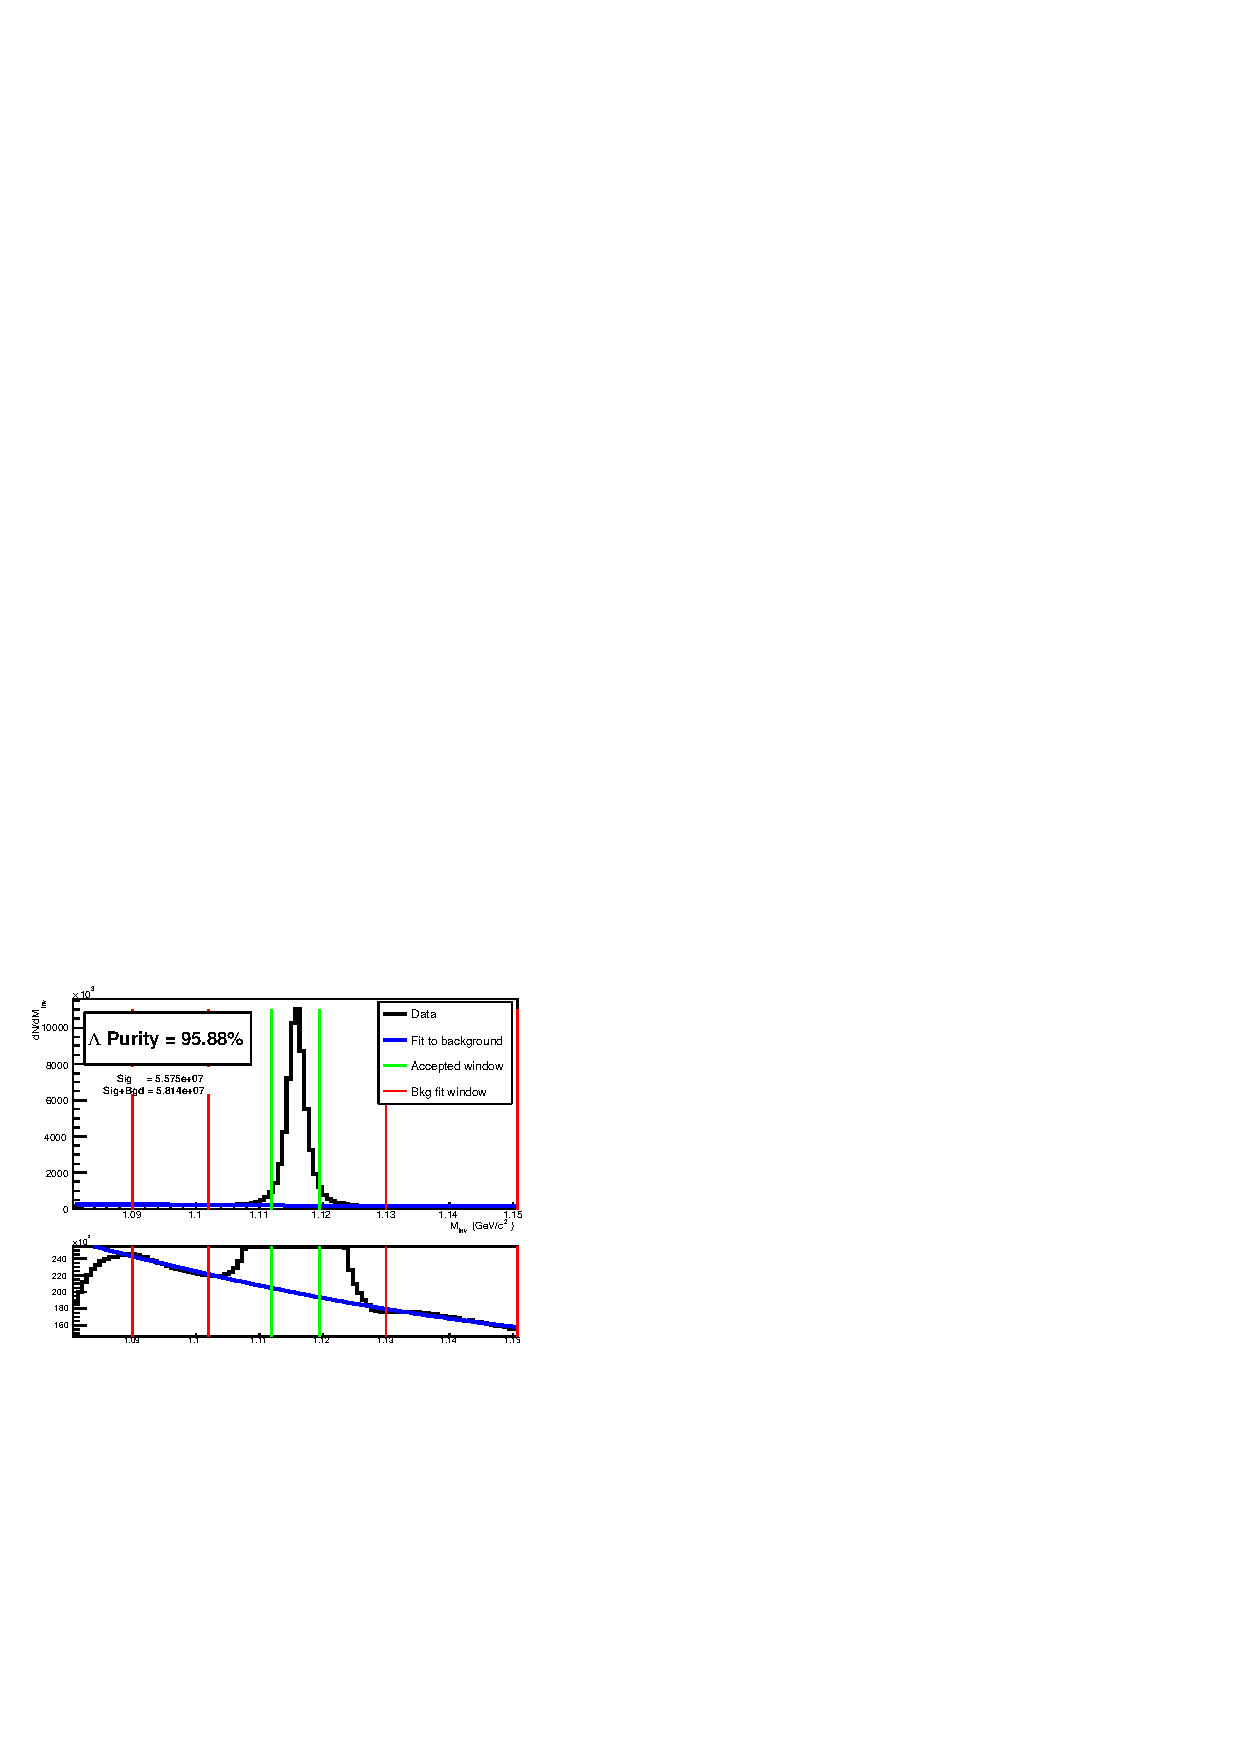
\includegraphics[width=0.49\linewidth]{/home/jesse/Analysis/FemtoAnalysis/LamKPublication/Figures/PDF/LamPurity_LamK0.pdf}}
  %%----start of second subfigure---  
  \subfigure[$\pi^{+}\pi^{-}$ invariant mass distribution where the \Ks peak is seen.]{
    \label{fig:Purity:b}
    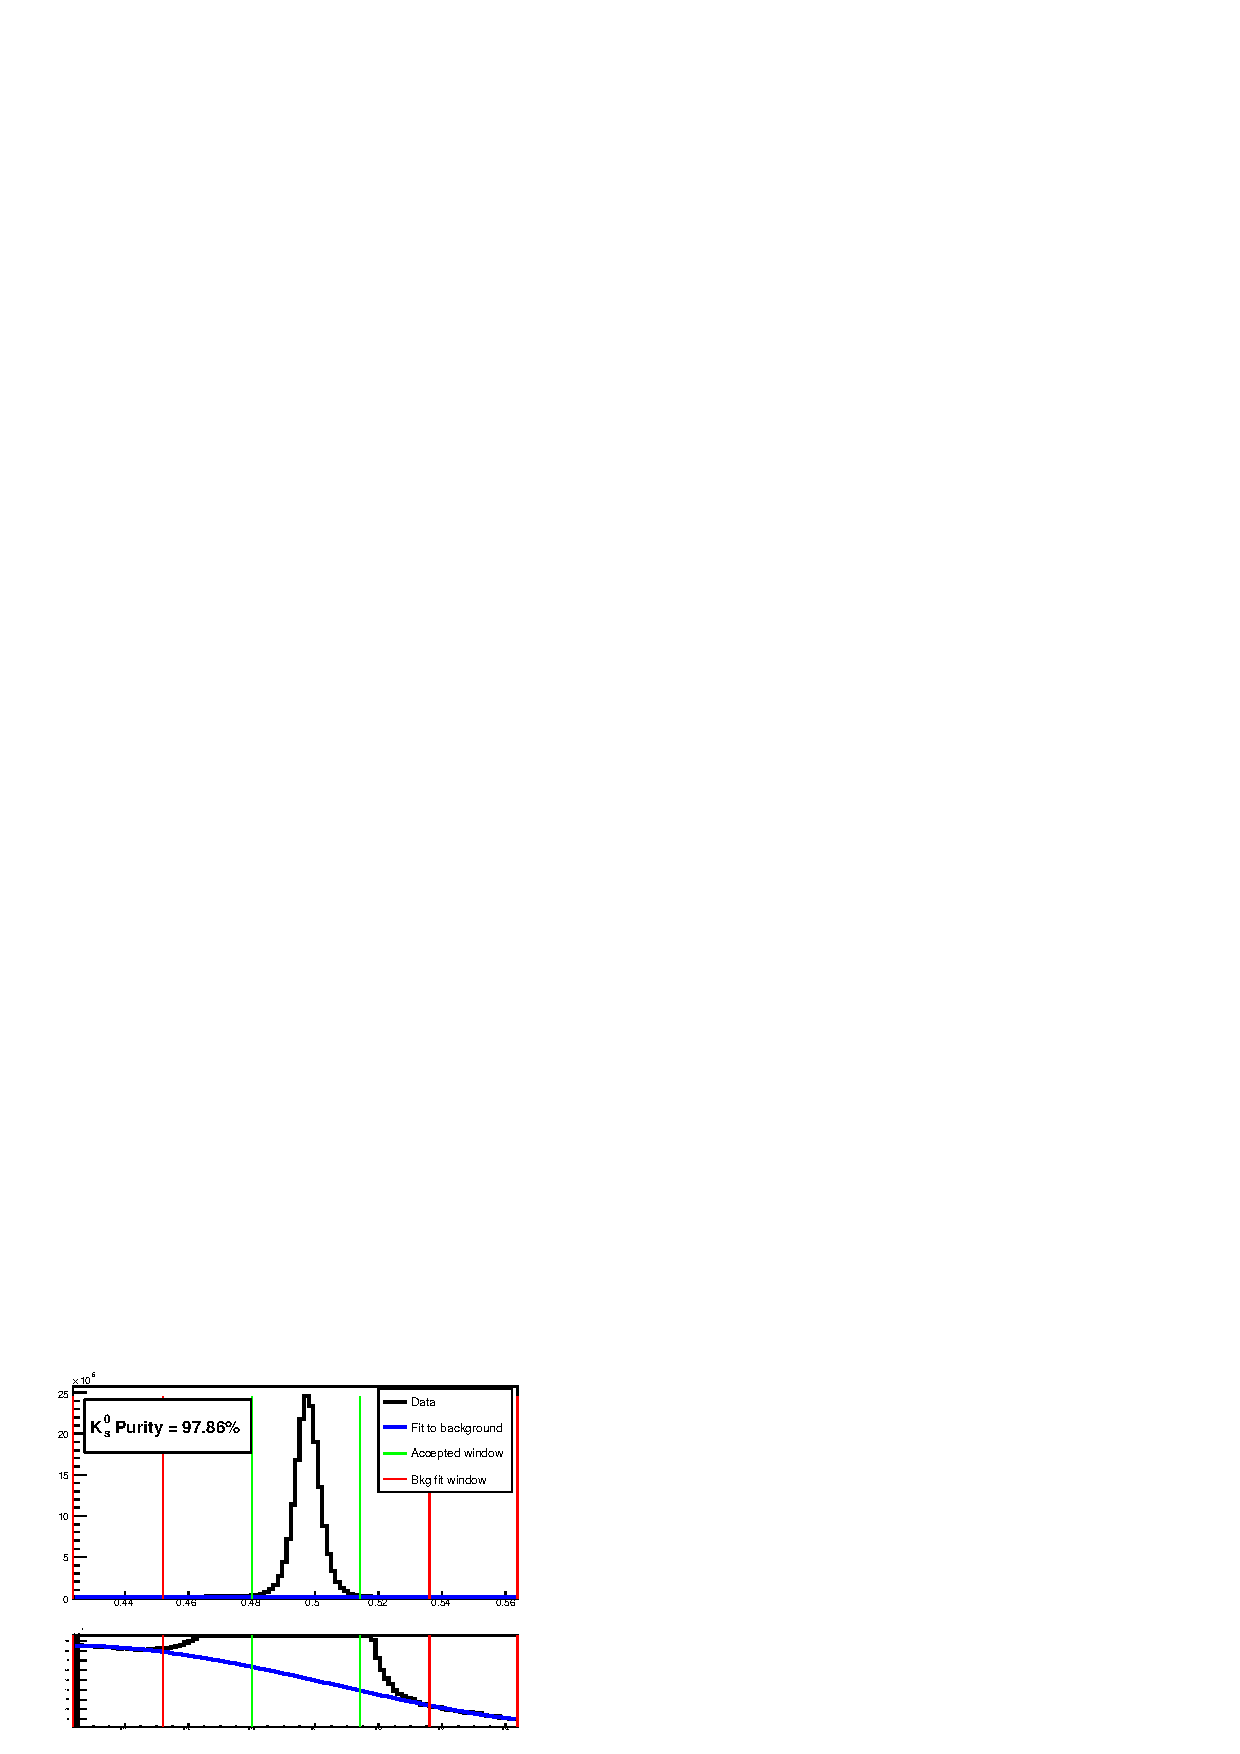
\includegraphics[width=0.49\linewidth]{/home/jesse/Analysis/FemtoAnalysis/LamKPublication/Figures/PDF/K0Purity_LamK0.pdf}}
  %%----overall caption----
  \caption{Invariant mass (m$_{\mathrm{inv}}$) distribution of all \Lam \ref{fig:Purity:a} and \Ks \ref{fig:Purity:b} candidates immediately before the final invariant mass cut.  The bottom figures are zoomed to show the background with fit.  The vertical green lines represent the m$_{\mathrm{inv}}$ cuts used in the analyses, the red vertical lines delineate the region over which the background was fit, and the blue line shows the background fit.  These distributions (or similar, for \ALam) are used to calculate the collection purities, Purity(\Lam) $\approx$ Purity(\ALam) $\approx$ 95\%, and Purity(\Ks) $\approx$ 98\%.}  
  \label{fig:Purity}
\end{figure}



\subsection{K$^{\pm}$ selection}
\label{sec:KchSelection}
The single-particle selection criteria used to select charged kaon candidates are summarized in Table \ref{tab:KchCuts}.
\Kpm identification utilized both TPC (what momenta?) and TOF (what momenta?).
Figure \ref{fig:KchPdEdx} shows d$E$/d$x$.

\begin{figure}[h]
 \centering
 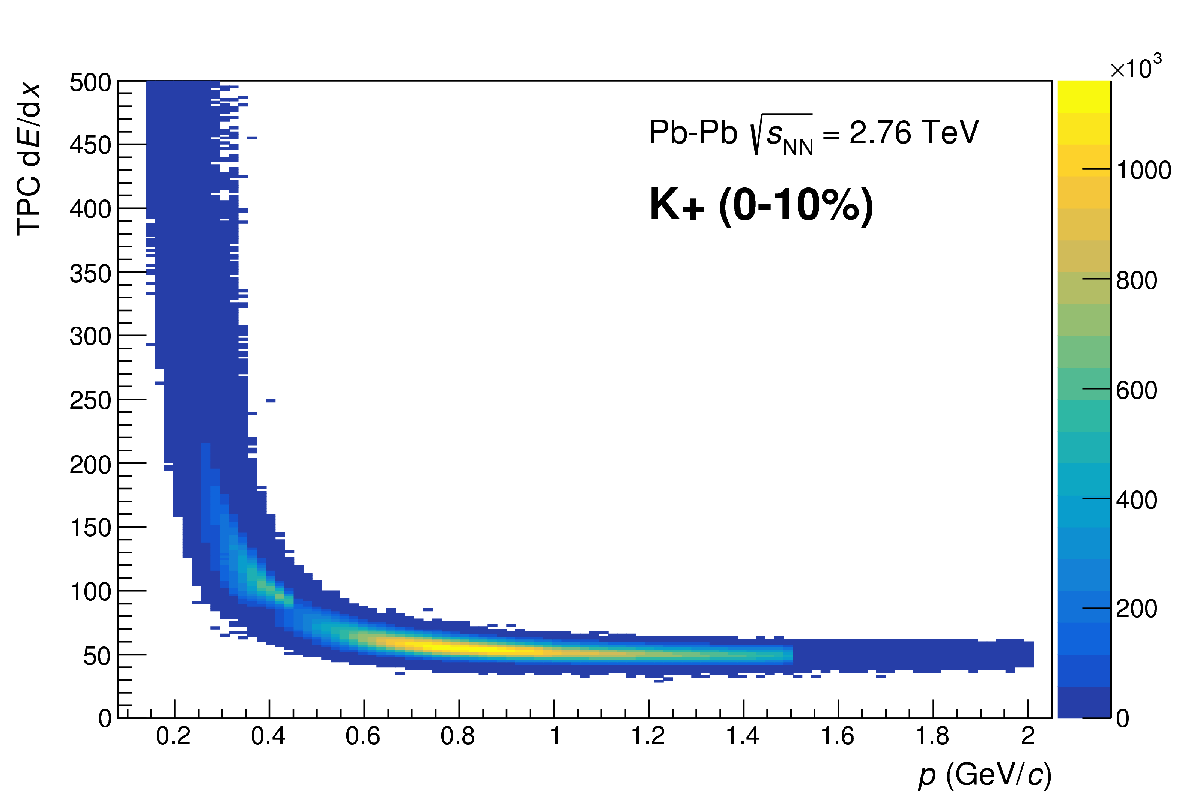
\includegraphics[width=1.0\textwidth]{/home/jesse/Analysis/FemtoAnalysis/LamKPublication/Figures/PDF/canDrawKchdEdx_LamKchP_0010_KchP.pdf}% Here is how to import EPS art
 \caption{\label{fig:KchPdEdx} A figure caption. The figure captions are
automatically numbered.}
\end{figure}

\begin{table}[htbp]
 \centering
%  \renewcommand{\arraystretch}{1.5}
  \begin{tabular}{lc|c|l}
   \hline  
   \multicolumn{4}{c}{\textbf{\Kpm selection}} \\
   \hline
   \multicolumn{3}{l|}{$|\eta|$} & $< 0.8$ \\
   \hline
   \multicolumn{3}{l|}{$p_{\mathrm{T}}$} & 0.14 $< p_{\mathrm{T}} < 1.5$ GeV/\textit{c} \\
   \hline
   \multicolumn{3}{l|}{FilterBit} & 7 \\
   \hline
   \multicolumn{3}{l|}{Min. number of clusters in the TPC} & 80 \\
   \hline
   \multicolumn{3}{l|}{Max. allowed $\chi^{2}/N_{DOF}$ for ITS clusters} & 3.0 \\
   \hline
   \multicolumn{3}{l|}{Max. allowed $\chi^{2}/N_{DOF}$ for TPC clusters} & 4.0 \\
   \hline   
   \multicolumn{3}{l|}{Maximum XY impact parameter} & 2.4 cm \\
   \hline
   \multicolumn{3}{l|}{Maximum Z impact parameter} & 3.0 cm \\
   \hline
   \multicolumn{3}{l|}{Remove particles with any kink labels} & true \\
   \hline
   \multicolumn{3}{l|}{Maximum allowed sigma to primary vertex} & 3.0 \\
   \hline   
   
   \multicolumn{4}{l}{PID Probabilities} \\
   \hline
    & \multicolumn{2}{l|}{K} & $>$ 0.2 \\
   \hline
    & \multicolumn{2}{l|}{$\pi$} & $<$ 0.1 \\
   \hline
    & \multicolumn{2}{l|}{$\mu$} & $<$ 0.8 \\
   \hline
    & \multicolumn{2}{l|}{p} & $<$ 0.1 \\
   \hline
   
   \multicolumn{3}{l|}{Most probable particle type} & Kaon (fMostProbable=3) \\
   \hline
   
   \multicolumn{4}{l}{TPC and TOF N$\sigma$ Cuts} \\
   \cline{2-4}
    & \multicolumn{1}{l}{$p <$ 0.4 GeV/\textit{c}} &  & N$_{\sigma \mathrm{K,TPC}} <$ 2 \\
   \cline{2-4}
    & \multicolumn{1}{l}{0.4 $< p <$ 0.45 GeV/\textit{c}} & & N$_{\sigma \mathrm{K,TPC}} <$ 1 \\
   \cline{2-4}     
    & \multicolumn{1}{l}{0.45 $< p <$ 0.80 GeV/\textit{c}} & & N$_{\sigma \mathrm{K,TPC}} <$ 3 \& N$_{\sigma \mathrm{K,TOF}} <$ 2 \\ 
   \cline{2-4}
    & \multicolumn{1}{l}{0.80 $< p <$ 1.0 GeV/\textit{c}} & & N$_{\sigma \mathrm{K,TPC}} <$ 3 \& N$_{\sigma \mathrm{K,TOF}} <$ 1.5 \\ 
   \cline{2-4}
    & \multicolumn{1}{l}{$p >$ 1.0 GeV/\textit{c}} & & N$_{\sigma \mathrm{K,TPC}} <$ 3 \& N$_{\sigma \mathrm{K,TOF}} <$ 1 \\ 
   \hline
   \multicolumn{3}{l|}{Electron Rejection} & Reject if N$_{\sigma e^{-},\mathrm{TPC}} < $ 3 \\
   \hline
   
   \multicolumn{4}{l}{Pion Rejection:  Reject if:} \\
   \hline
   \multirow{3}{*}{$p <$ 0.65 GeV/\textit{c}} & if TOF and TPC available & \multicolumn{1}{c}{} & N$_{\sigma \pi,\mathrm{TPC}} <$ 3 \& N$_{\sigma \pi,\mathrm{TOF}} <$ 3 \\
   \cline{2-4}
    & \multirow{2}{*}{else} & $p <$ 0.5 GeV/\textit{c} & N$_{\sigma \pi,\mathrm{TPC}} <$ 3 \\
   \cline{3-4}
    &  & 0.5 $< p <$ 0.65 GeV/\textit{c} & N$_{\sigma \pi,\mathrm{TPC}} <$ 2 \\
   \cline{2-4}
   \multicolumn{3}{l|}{0.65 $< p <$ 1.5 GeV/\textit{c}} & N$_{\sigma \pi,\mathrm{TPC}} <$ 5 \& N$_{\sigma \pi,\mathrm{TOF}} <$ 3 \\
   \cline{2-4}
   \multicolumn{3}{l|}{$p >$ 1.5 GeV/\textit{c}} & N$_{\sigma \pi,\mathrm{TPC}} <$ 5 \& N$_{\sigma \pi,\mathrm{TOF}} <$ 2 \\
   \hline
  \end{tabular}
% \end{minipage}
 \caption{\Kpm selection}
 \label{tab:KchCuts} 
\end{table}

The purity of the \Kpm collections was estimated using the MC data, for which the true identity of each reconstructed K$^{\pm}$ particle is known.  Therefore, the purity may be estimated as:

\begin{equation}
 Purity(K^{\pm}) = \frac{N_{true}}{N_{reconstructed}} \\
\label{eqn:KchPurity}
\end{equation}

Purity(\KchP) $\approx$ Purity(\KchM) $\approx$ 97\%


\subsection{Pair Selection}
\label{PairSelection}
I suppose I should probably briefly explain how pairs are formed?

It is important to obtain true particle pairs in the analysis.  In particular, contamination from pairs constructed with split or merged tracks, and pairs sharing daughters, can introduce an artificial signal into the correlation function, obscuring the actual physics.  In an effort to remove contamination, we impose two main two-particle cuts: a shared daughter cut, and an average separation cut.  

The purpose of the shared daughter cut is to ensure the first particle in the pair is unique from the second.  For pairs formed of two V0s (i.e. \LamKs), this cut is implemented by removing all pairs which share a daughter (ex. in \LamKs analysis, if the \Lam and \Ks in a potential pair claim the same $\pi^{-}$ daughter, the pair is excluded from the analysis).  For a pair formed of a single V0 and a charged track (i.e. \LamKpm), the cut removes all pairs in which the charged track is also claimed as a daughter of the V0.  This mistake could only occur if, for instance, a \Kpm is misidentified as a $\pi$ or p either in the V0 reconstruction or in the \Kpm selection.

The purpose of the average separation cut in to remove splitting and merging effects.  How do we estimate the cut values?  How do we implement the cut?

For the \LamALamKs analysis, the average separation for like-charge daughters must be greater than 6.0 cm.  We enforce no cut for unlike-charge daughters.  For example, we impose this cut in a \LamKs analysis on the p daughter of the \Lam and the $\pi^{+}$ daughter of the \Ks.  For the \LamKpm analyses, the average separation between the \LamALam daughter (sharing the same charge as the \Kpm) and the \Kpm is 8.0 cm.  We enforce no cut for unlike signs.  For a \LamKchP analysis, we impose this cut between the p daughter of the \Lam and the \KchP in the pair.








\section{Construction of correlation functions and fitting}
\label{sec:CfConstructionAndFitting}
The event mixing was handled by the AliFemtoVertexMultAnalysis class, which only mixes events with like vertex position and centrality.
The following criteria were used for event mixing:

\begin{itemize}
 \itemsep0em
 \item Number of events to mix = 5
 \item Vertex position bin width = 2 cm
 \item Centrality bin width = 5%
\end{itemize}


%General remarks about formaton of correlation functions and what information they provide.

This analysis studies the momentum correlations of both \LamK and $\Xi$K pairs using the two-particle correlation function, defined as $C(k^{*}) = A(k^{*})/B(k^{*})$, where $A(k^{*})$ is the signal distribution, $B(k^{*})$ is the reference (or background) distribution, and $k^{*}$ is the momentum of one of the particles in the pair rest frame.
In practice, $A(k^{*})$ is constructed by binning in \kst pairs from the same event.
Ideally, $B(k^{*})$ is similar to $A(k^{*})$ in all respects excluding the presence of femtoscopic correlations \cite{Lisa:2005dd}; as such, $B(k^{*})$ is used to divide out the phase-space effects, leaving only the femtoscopic effects in the correlation function. 

In practice, $B(k^{*})$ is obtained by forming mixed-event pairs, i.e. particles from a given event are paired with particles from N$_{mix}$(= 5) other events, and these pairs are then binned in \kst.
In forming the background distribution, it is important to mix only similar events; mixing events with different phase-spaces can lead to artificial signals in the correlaton function.
Therefore, in this analysis, we mix events with primary vertices within 2 cm and centralities within 5\% of each other.
Also note, a vertex correction is also applied to each event, which essentially recenters the the primary vertices to z = 0.

This analysis presents correlation functions for three centrality bins (0-10\%, 10-30\%, and 30-50\%), and is currently pair transverse momentum ($k_{\mathrm{T}} = 0.5|\mathbf{p}_{\mathrm{T,1}}+\mathbf{p}_{\mathrm{T,2}}|$) integrated (i.e. not binned in $k_{T}$).  
The correlation functions are constructed separately for the two magnetic field configurations, and are combined using a weighted average:

\begin{equation}
  C_{combined}(k^{*}) = \frac{\sum\limits_{i}w_{i}C_{i}(k^{*})}{\sum\limits_{i}w_{i}} 
\label{eqn:CombineCfs}
\end{equation}

where the sum runs over the correlation functions to be combined, and the weight, $w_{i}$, is the number of numerator pairs in $C_{i}(k^{*})$.
Here, the sum is over the two field configurations.

Figures \ref{fig:LamKFits_3Res:a}, \ref{fig:LamKFits_3Res:b}, and \ref{fig:LamKFits_3Res:c} show the correlation functions for all centalities studied for \LamKchPALamKchM, \LamKchMALamKchP, and \LamKsALamKs, respectively. All were normalized in the range 0.32 $< k^{*} < $ 0.4 GeV/$c$.


\subsection{Fit Function}
\label{sec:FitFunction}
Ya boys Lednicky and Lyuboshitz!

The two-particle relative momentum correlation function may be written theoretically by the Koonin-Pratt equation \cite{Koonin:1977fh, Pratt:1990zq}:

\begin{equation}
 C(\mathbf{k^{*}}) = \int S(\mathbf{r^{*}})|\Psi_{\mathbf{k^{*}}}(\mathbf{r^{*}})|^{2}d^{3}\mathbf{r^{*}}
\label{eqn:KooninPrattEqn}
\end{equation}

In the absence of Coulomb effects, and assuming a spherically gaussian source of width $R$, the 1D femtoscopic correlation function can be calculated analytically using:

\begin{equation}
 C(k^{*}) = 1 + C_{QI}(k^{*}) + C_{FSI}(k^{*})
\label{eqn:LednickyEqn}
\end{equation}

$C_{QI}$ describes plane-wave quantum interference:

\begin{equation}
 C_{QI}(k^{*}) = \alpha\exp(-4k^{*2}R^{2})
\label{eqn:CQI}
\end{equation}

where $\alpha = (-1)^{2j}/(2j+1)$ for identical particles with spin j, and $\alpha = 0$ for non-identical particles.  Obviously, $\alpha = 0$ for all analyses presented in this note.  $C_{FSI}$ describes the s-wave strong final state interaction between the particles:

\begin{equation}
\begin{array}{l}
\vspace{2mm}  %%space between C_{FSI}(k^{*}) and f(k^{*})
  C_{FSI}(k^{*}) = (1+\alpha)[\frac{1}{2}|\frac{f(k^{*})}{R}|^2(1-\frac{d_{0}}{2\sqrt{\pi}R})+\frac{2\mathbb{R}f(k^{*})}{\sqrt{\pi}R}F_{1}(2k^{*}R)-\frac{\mathbb{I}f(k^{*})}{R}F_{2}(2k^{*}R)] \\
\vspace{2mm}  %%space after f(k^{*})  
  ~~~~~f(k^{*}) = (\frac{1}{f_{0}}+\frac{1}{2}d_{0}k^{*2}-ik^{*})^{-1};~~~
  F_{1}(z) = \int_{0}^{z} \frac{e^{x^{2}-z^{2}}}{z}dx;~~~
  F_{2}(z) = \frac{1-e^{-z^{2}}}{z}
\end{array}  
\label{eqn:CFSI}
\end{equation}

where $R$ is the source size, $f(k^{*})$ is the s-wave scattering amplitude, $f_{0}$ is the complex scattering length, and $d_{0}$ is the effective range of the interaction.

An additional parameter $\lambda$ is typically included in the femtoscopic fit function to account for the purity of the pair sample.  In the case of no residual correlations (to be discussed in Section \ref{ResidualCorrelations}, the fit function becomes:

\begin{equation}
 C(k^{*}) = 1 + \lambda[C_{QI}(k^{*}) + C_{FSI}(k^{*})]
\label{eqn:LednickyEqnwLambda}
\end{equation}




The two-particle correlation function may be written as:

\begin{equation}
 C(\mathbf{k^{*}}) = \sum\limits_{S}\rho_{S}\int S(\mathbf{r^{*}})|\Psi^{S}_{\mathbf{k^{*}}}(\mathbf{r^{*}})|^{2}d^{3}\mathbf{r^{*}}
\label{eqn:GenCfEqn}
\end{equation}

where $\rho_{S}$ is the normalized emission probability of particles in a state with spin S, $S(\mathbf{r}^{*})$ is the pair emission source distribution (assumed to be Gaussian), and $\Psi^{S}_{\mathbf{k}^{*}}(\mathbf{r}^{*})$ is the two-particle wave-function including both strong and Coulomb interactions \cite{Lednicky:2005tb}:

\begin{equation}
 \Psi_{\mathbf{k^{*}}}(\mathbf{r^{*}}) = e^{i\delta_{c}}\sqrt{A_{c}(\eta)}[e^{i\mathbf{k^{*}} \cdot \mathbf{r^{*}}}F(-i\eta,1,i\xi) + f_{c}(k^{*})\frac{\tilde{G}(\rho,\eta)}{r^{*}}]
\label{eqn:CoulombWaveFcn}
\end{equation}

where $\rho = k^{*}r^{*}$, $\eta = (k^{*}a_{c})^{-1}$, $\xi = \mathbf{k^{*}} \cdot \mathbf{r^{*}} + k^{*}r^{*} \equiv \rho(1+\cos\theta^{*})$, and $a_{c} = (\mu z_{1}z_{2}e^{2})^{-1}$ is the two-particle Bohr radius (including the sign of the interaction).  $\delta_{c}$ is the Coulomb s-wave phase shift, $A_{c}(\eta)$ is the Coulomb penetration factor, $\tilde{G} = \sqrt{A_{c}}(G_{0} + iF_{0})$ is a combination of the regular ($F_{0}$) and singular ($G_{0}$) s-wave Coulomb functions.  $f_{c}(k^{*})$ is the s-wave scattering amplitude:

\begin{equation}
 f_{c}(k^{*}) = [\frac{1}{f_{0}} + \frac{1}{2}d_{0}k^{*2} - \frac{2}{a_{c}}h(\eta) - ik^{*}A_{c}(\eta)]^{-1}
\label{eqn:CoulombScattAmp}
\end{equation}

where, the ``h-function", $h(\eta$), is expressed through the digamma function, $\psi(z)$ = $\Gamma'(z)/\Gamma(z)$ as:

\begin{equation}
 h(\eta) = 0.5[\psi(i\eta) + \psi(-i\eta) - \ln(\eta^{2})]
\label{eqn:LednickyHFunction}
\end{equation} 

In this case, the $\lambda$ parameter may be included as: 

\begin{equation}
 C(\mathbf{k^{*}}) = (1 - \lambda) + \lambda\sum\limits_{S}\rho_{S}\int S(\mathbf{r^{*}})|\Psi^{S}_{\mathbf{k^{*}}}(\mathbf{r^{*}})|^{2}d^{3}\mathbf{r^{*}}
\label{eqn:GenCfEqnwLambda}
\end{equation}


\subsection{Momentum Resolution Corrections}
\label{MomentumResolutionCorrections}

Finite track momentum resolution causes the reconstructed momentum of a particle to smear around the true value.
This, of course, also holds true for V0 particles.
The effect is propagated up to the pairs of interest, which causes the reconstructed relative momentum ($k^{*}_{Rec}$) to differ from the true momentum ($k^{*}_{True}$).
Smearing of the momentum typically will result in a suppression of the signal.

The effect of finite momentum resolution can be investigated using the MC data, for which both the true and reconstructed momenta are available.

Information gained from looking at $k^{*}_{Rec}$ vs $k^{*}_{True}$ can be used to apply corrections to account for the effects of finite momentum resolution on the correlation functions.



A second approach is to use information gained from response matrices.
The response matrix describes quantitatively how each $k^{*}_{Rec}$ bin receives contributions from multiple $k^{*}_{True}$ bins, and can be used to account for the effects of finite momentum resolution.
With this approach, the resolution correction is applied on-the-fly during the fitting process by propagating the theoretical (fit) correlation function through the response matrix, according to:  

\begin{equation}
  C_{fit}(k^{*}_{Rec}) = \dfrac{\sum\limits_{k^{*}_{True}}M_{k^{*}_{Rec},k^{*}_{True}}C_{fit}(k^{*}_{True})}{\sum\limits_{k^{*}_{True}}M_{k^{*}_{Rec},k^{*}_{True}}}
\label{eqn:MomResCorrection}
\end{equation}

where $M_{k^{*}_{Rec},k^{*}_{True}}$ is the response matrix, $C_{fit}(k^{*}_{True})$ is the fit binned in $k^{*}_{True}$, and the denominator normalizes the result.

Equation \ref{eqn:MomResCorrection} describes that, for a given $k^{*}_{Rec}$ bin, the observed value of $C(k^{*}_{Rec})$ is a weighted average of all $C(k^{*}_{True})$ values, where the weights are the normalized number of counts in the [$k^{*}_{Rec}$, $k^{*}_{True}$] bin.




\subsection{Residual Correlations}
\label{ResidualCorrelations}

The purpose of this analysis is study the interaction and scale of the emitting source of the pairs.
In order to obtain correct results, it is important for our particle collections to consist of primary particles.
In practice, this is difficult to achieve for our $\Lambda$ and $\bar{\Lambda}$ collections.
Many of our $\Lambda$ particles are not primary, but originate as decay products from other hyperons, including $\Sigma^{0}$, $\Xi^{0}$, $\Xi^{-}$ and $\Sigma^{*(+,-,0)}(1385)$.  Additionally, many of our K particles are not primary, but decay from K$^{*(+,-,0)}(892)$ parents.
In these decays, the $\Lambda$ carries away a momentum very similar to that of its parent.
As a result, the correlation function between a secondary $\Lambda$ and, for instance, a K$^{+}$  will be sensitive to, and dependent upon, the interaction between the parent of the $\Lambda$ and the K$^{+}$.
In effect, the correlation between the parent of the $\Lambda$ and the K$^{+}$ (ex. $\Sigma^{0}$K$^{+}$) will be visible, although smeared out, in the $\Lambda$K$^{+}$ data.
We call this a residual correlation resulting from feed-down.  Residual correlations are important in an analysis when three criteria are met \cite{Kisiel:2014mma}: i) the parent correlation signal is large, ii) a large fraction of pairs in the sample originate from the particular parent system, and iii) the decay momenta are comparable to the expected correlation width in \textit{k}*. 

As it is difficult for us to eliminate these residual correlations in our analyses, we must attempt to account for them in our fitter.
To achieve this, we will simultaneously fit the data for both the primary correlation function and the residual correlations.  For example, in the simple case of a $\Lambda$K$^{+}$ analysis with residuals arising solely from $\Sigma^{0}$K$^{+}$ feed-down:

\begin{equation}
\begin{array}{l}
\vspace{4mm}
 C_{measured}(k^{*}_{\Lambda K^{+}}) = 1 + \lambda_{\Lambda K^{+}}[C_{\Lambda K^{+}}(k^{*}_{\Lambda K^{+}})-1] + \lambda_{\Sigma^{0}K^{+}}[C_{\Sigma^{0}K^{+}}(k^{*}_{\Lambda K^{+}})-1] \\
\vspace{2mm}
  ~~~~~C_{\Sigma^{0}K^{+}}(k^{*}_{\Lambda K^{+}}) \equiv \frac{\sum\limits_{k^{*}_{\Sigma^{0}K^{+}}} C_{\Sigma^{0}K^{+}}\left(k^{*}_{\Sigma^{0}K^{+}}\right) T\left(k^{*}_{\Sigma^{0}K^{+}},k^{*}_{\Lambda K^{+}}\right)}{\sum\limits_{k^{*}_{\Sigma^{0}K^{+}}} T\left(k^{*}_{\Sigma^{0}K^{+}},k^{*}_{\Lambda K^{+}}\right)}
\end{array} 
\label{eqn:SimpleResiduals}
\end{equation}

$C_{\Sigma^{0}K^{+}}(k^{*}_{\Sigma^{0}K^{+}})$ is the $\Sigma^{0}$K$^{+}$ correlation function from, for instance, Equation \ref{eqn:LednickyEqn}, and $T$ is the transform matrix generated with THERMINATOR.  The transform matrix is formed for a given parent pair, AB, by taking all $\Lambda$K pairs originating from AB, calculating the relative momentum of the parents (\textit{k}*$_{AB}$) and daughters (\textit{k}*$_{\Lambda K}$), and filling a two-dimensional histogram with the values. The transform matrix is essentially an unnormalized probability distribution mapping the \textit{k}* of the parent pair to that of the daughter pair when one or both parents decay.

  The above equation can be easily extended to include feed-down from more sources:

\begin{equation}
\begin{array}{l}
\vspace{4mm}
\begin{split}
 C_{measured}(k^{*}_{\Lambda K}) & = 1 + \lambda_{\Lambda K}[C_{\Lambda K}(k^{*}_{\Lambda K})-1] + \lambda_{\Sigma^{0}K}[C_{\Sigma^{0}K}(k^{*}_{\Lambda K})-1] + ... \\ &
 + \lambda_{P_{1}P_{2}}[C_{P_{1}P_{2}}(k^{*}_{\Lambda K})-1] + \lambda_{other}[C_{other}(k^{*}_{\Lambda K})-1] 
\end{split}
\\
\vspace{2mm}
  ~~~~~C_{P_{1}P_{2}}(k^{*}_{\Lambda K}) \equiv \frac{\sum\limits_{k^{*}_{P_{1}P_{2}}} C_{P_{1}P_{2}}\left(k^{*}_{P_{1}P_{2}}\right) T\left(k^{*}_{P_{1}P_{2}},k^{*}_{\Lambda K}\right)}{\sum\limits_{k^{*}_{P_{1}P_{2}}} T\left(k^{*}_{P_{1}P_{2}},k^{*}_{\Lambda K}\right)}
\end{array} 
\label{eqn:ResidualsFull}
\end{equation}

  Or, more compactly:

\begin{equation}
 C_{measured}(k^{*}_{\Lambda K}) = 1 + \sum\limits_{i}  \lambda_{i}[C_{i}(k^{*}_{\Lambda K})-1]
\label{eqn:Residuals}
\end{equation}



So, in practice, we model the correlation function of the parents, and run the correlation function through the appropriate transform matrix to determine the contribution to the daughter correlation function.  A few questions still remain.  First, what $\lambda$ values should be used in the above equation?  One option would be to leave all of these $\lambda$-parameters free during the fit process.  However, this would introduce a huge number of new parameters into the fitter, and would make the fit results less trustworthy.  The $\lambda$ parameters roughly dictate the strength of the parent contribution to the daughter pair.  Additionally, as found in \cite{Salzwedel:2241303}, the reconstruction efficiency for primary $\Lambda$ particles is nearly equal to that of $\Lambda$ particles originating from $\Sigma$, $\Sigma^{*}$, $\Xi^{0}$, $\Xi^{-}$, and $\Omega$ hyperons.  Therefore, the $\lambda$ parameter for parent system AB can be estimated using THERMINATOR as the total number of $\Lambda$K pairs originating from AB (N$_{AB}$) divided by the total number of $\Lambda$K pairs (N$_{Total}$): 

\begin{equation}
\lambda_{AB} = \frac{N_{AB}}{N_{Total}}
\end{equation}




Now, the remaining question is how do we model the parent correlation functions?  In an ideal world, we would simply look up the parent interaction in some table, and input this into our model.  Unfortunately, the world in which we live is not perfect, such a table does not exists, and little is know about the interaction between the particles in the residual pairs of this study.  One solution would be to introduce a set of scattering parameters and radii for each residual system.  However, as will the case of the $\lambda$-parameters above, this would introduce a large number of additional fit parameters, and would make our fitter too unconstrained and would yield untrustworthy results.  The second option, which is adopted in this analysis, is to assume all residual pairs have the same source size as the daughter pair, and all Coulomb-neutral residual pairs also share the same scattering parameters as the daughter pair (the case of charged pairs will be described below).



Now, as hinted above, accounting for charged residuals adds a complication in that they necessitate the inclusion of the CoulombFitter into the process.  We have two solutions to bypass such a large increase in run time.  First, we can use our experimental $\Xi^{\mathrm{ch}}$K$^{\mathrm{ch}}$ data to represent all charged parent pair system.  In this case, there is no need to make any assumption about scattering parameters or source sizes, as we already have the experimental data.  The downside is that, especially in the 30-50\% centrality bin, the error bars on the data are large.  Alternatively, we can assume the strong interaction is negligible in the charged residual, and generate the parent correlation function given radius and $\lambda$ parameters.  We find in our $\Xi^{\mathrm{ch}}$K$^{\mathrm{ch}}$ study that a Coulomb-only description of the system describes, reasonably well, the broad features of the correlation.  The strong interaction is necessary for the fine details.  However, as these correlations are run through a transform matrix, which largely flattens out and fine details, a Coulomb-only description should be sufficient.  We find consistent results between using the $\Xi$K data and the Coulomb-only interpolation method.  When the number of residual pairs used is increased to 10, so that pairs such as $\Sigma^{*+}$K$^{-}$ enter the picture, the Coulomb-only interpolation method is used.  In other words, the $\Xi$K experimental data is only used to model the $\Xi$K residual contribution, all other charged pairs are treated with the Coulomb-only interpolation method.


\subsection{Non-Flat Background}
\label{NonFlatBackground}


Non-flat background
Adam's paper \cite{Kisiel:2017}.




\subsection{LednickyFitter}
\label{LednickyFitter}


A simple $\chi^{2}$ test is inappropriate for fitting correlation functions, as the ratio two Poisson distributions does not result in a Poisson distribution.
Instead, a log-likelihood fit function of the following form is used \cite{Lisa:2005dd}:

\begin{equation}
 \chi^{2}_{PML} = -2\left[A\ln\left(\frac{C(A+B)}{A(C+1)}\right) + B\ln\left(\frac{A+B}{B(C+1)}\right)\right]
\label{eqn:Chi2PML}
\end{equation}

where $A$ is the experimental signal distribution (numerator), $B$ is the experimental background distribution (denominator), and $C$ is the theoretical fit correlation function.

The fitter uses Equations \ref{eqn:LednickyEqn} -- \ref{eqn:CFSI} to build the theoretical fit, and Equation \ref{eqn:Chi2PML} as the statistic quantifying the quality of the fit.
The parameters of the fit are: $\lambda$, $R$, $f_{0}$ ($\mathbb{R}f_{0}$ and $\mathbb{I}f_{0}$ separately), $d_{0}$, and normalization $N$.
The fitter currently includes methods to correct for momentum resolution and a non-flat background.
These corrections are applied to the fit function, the data is never touched.
The fitter is able to share parameters between different analyses and fit all simultaneously.  

In a typical fit, a given pair is fit with its conjugate (ex. $\Lambda$K$^{+}$ with $\bar{\Lambda}$K$^{-}$) across all centralities (0-10\%, 10-30\%, 30-50\%), for a total of 6 simultaneous analyses.
Each analysis has a unique $\lambda$ and normalization parameter.
The radii are shared between analyses of like centrality, as these should have similar source sizes.
The scattering parameters ($\mathbb{R}f_{0}$, $\mathbb{I}f_{0}$, $d_{0}$) are shared amongst all.

In the case of fitting with residuals, the $\lambda_{Fit}$ parameter serves as an overall normalization shared by all contributors, such that Eqn \ref{eqn:Residuals} becomes:

\begin{eqnarray}
 C_{measured}(k^{*}_{\Lambda K}) &=& 1 + \sum\limits_{i}\lambda_{i}'[C_{i}(k^{*}_{\Lambda K})-1] \\
 \lambda_{i}' &=& \lambda_{Fit}\lambda_{i} \notag \\
 \sum\limits_{i}\lambda_{i}' &=&  \lambda_{Fit}\sum\limits_{i}\lambda_{i} = \lambda_{Fit} \notag
\label{eqn:ResidualsvLambdaNorm} 
\end{eqnarray}

where $\lambda_{i}$ is obtained from THERMINATOR, as explained in Section \ref{ResidualCorrelations}, and whose values are presented in Tables \ref{tab:LambdaValues_LamKchP} through \ref{tab:LambdaValues_LamK0}.  For Coulomb-neutral pairs, such as $\Lambda$K, $\Sigma^{0}$K, and $\Xi^{0}$K, $C_{i}(k^{*}_{\Lambda K})$ is calculated from Eqn. \ref{eqn:LednickyEqn}, with the help of Eqn. \ref{eqn:CFSI}.  For those residual pairs which include a Coulomb interaction, $C_{i}(k^{*}_{\Lambda K})$ is either calculated assuming no strong interaction, or by using the $\Xi^{\mathrm{ch}}\mathrm{K^{ch}}$ data directly.  Unless otherwise stated, the $\Xi^{\mathrm{ch}}\mathrm{K^{ch}}$ residual contribution is modeled using the experimental $\Xi^{\mathrm{ch}}\mathrm{K^{ch}}$ data, and all other charged contributors (ex. $\Sigma^{*\mathrm{ch}}\mathrm{K^{ch}}$) are modeled using the Coulomb-only technique with no strong interaction contribution.

To summarize, the complete fit function is constructed as follows:

\begin{enumerate}
 \item The uncorrected correlation function, $C'_{Fit}(k^{*}_{True})$, is constructed using Eq. \ref{eqn:ResidualsvLambdaNorm}
 \begin{itemize}
 \item in the case of no residual contributions included in the fit, $\lambda_{i}$ = $\lambda_{\Lambda\mathrm{K}}$ in Eq. \ref{eqn:ResidualsvLambdaNorm} is set equal to 1.  Then, the extracted $\lambda_{Fit}$ parameter should be roughly equal to the pair purity.
 \end{itemize}
 \item The correlation function is corrected to account for momentum resolution effects using Eq. \ref{eqn:MomResCorrection}
 \begin{itemize}
  \item $C'_{fit}(k^{*}_{Rec}) = \dfrac{\sum\limits_{k^{*}_{True}}M_{k^{*}_{Rec},k^{*}_{True}}C'_{fit}(k^{*}_{True})}{\sum\limits_{k^{*}_{True}}M_{k^{*}_{Rec},k^{*}_{True}}}$
 \end{itemize}
 \item Finally, the non-flat background correction is applied, and the final fit function is obtained
 \begin{itemize}
  \item $C_{Fit}(k^{*}_{Rec}) = C'_{Fit}(k^{*}_{Rec})*F_{Bgd}(k^{*}_{Rec})$
 \end{itemize}
\end{enumerate}



\subsection{Coulomb Fitter}
\label{CoulombFitter}

When modeling systems which include both strong and Coulomb effects, Eq. \ref{eqn:LednickyEqn} is no longer valid, and, in fact, there is no analytical form with which to fit.
Therefore, we must begin with the wave function describing the pair interaction, and simulate many particle pairs to obtain a theoretical fit correlation function.
Unfortunately, the nature of this process means that the run time increases dramatically.


As stated before, to generate a fit correlation function, we must simulate a large number of pairs, calculate the wave-function, and average $\Psi^{2}$ over all pairs in a given k$^{*}$ bin.  Essentially, we calculate Equation \ref{eqn:GenCfEqn} by hand:

\begin{equation}
\begin{array}{l}
\vspace{2mm}
  C(\mathbf{k^{*}}) = \sum\limits_{S}\rho_{S}\int S(\mathbf{r^{*}})|\Psi^{S}_{\mathbf{k^{*}}}(\mathbf{r^{*}})|^{2}d^{3}\mathbf{r^{*}} \\
\vspace{2mm}
  \longrightarrow C(|\mathbf{k^{*}}|) \equiv C(k^{*}) = \sum\limits_{S}\rho_{S}\langle |\Psi^{S}(\mathbf{k^{*}_{i}},\mathbf{r^{*}_{i}})|^{2} \rangle_{i} \\
\vspace{2mm}
  \longrightarrow C(k^{*}) = \lambda\sum\limits_{S}\rho_{S}\langle |\Psi^{S}(\mathbf{k^{*}_{i}},\mathbf{r^{*}_{i}})|^{2} \rangle_{i} + (1-\lambda)

\end{array}
\label{eqn:CoulombEqn2}
\end{equation}

where $\langle \rangle_{i}$ represents an average over all pairs in a given k$^{*}$ bin.

In summary, for a given k$^{*}$ bin, we must draw $N_{pairs} \sim 10^{4}$ pairs, and for each pair:

\begin{enumerate}
 \item Draw a random $\mathbf{r}^{*}$ vector according to our Gaussian source distribution $S(\mathbf{r}^{*})$
 \item Draw a random $\mathbf{k}^{*}$ vector satisfying the $|\mathbf{k}^{*}|$ restriction of the bin
 \begin{itemize}
  \item We draw from real $k^{*}$ vectors obtained from the data
  \item However, we find that drawing from a distribution flat in $k^{*}$ gives similar results
 \end{itemize}
 \item Construct the wave-function $\Psi$
\end{enumerate}

After all pairs for a given k$^{*}$ bin are simulated and wave-functions obtained, the results are averaged to give the fit result.



\section{Systematic uncertainties}
\label{sec:SysErrs}

In order to understand my systematic uncertainties, the analysis code was run many times using slightly different values for a number of important cuts, and the results were compared.

In order to quantify the systematic errors on the data, all correlation functions built using all varied cut values were bin-by-bin averaged, and the resulting variance of each bin was taken as the systematic error.  The cuts which were utilized in this study are presented in Sections \ref{SysErrsLamK0:ParticleAndPairCuts} (\LamKs) and \ref{SysErrsLamKch:ParticleAndPairCuts} (\LamKpm).


Similarly, the fit parameters extracted from all of these correlation functions were averaged, and the resulting variances were taken as the systematic errors for the fit parameters.
As with the systematic errors on the data, this was performed for all varied cut values.
Additionally, a systematic analysis was done on our fit method.
These two sources of uncertainty were combined in quadrature to obtain the final systematic uncertainties on the extracted fit parameters.



\subsection{Systematic Errors: \texorpdfstring{$\Lambda$K$^{0}_{S}$}{TEXT}}
\label{SysErrsLamK0}

\subsubsection{Particle and Pair Cuts}
\label{SysErrsLamK0:ParticleAndPairCuts}

The cuts included in the systematic study, as well as the values used in the variations, are listed below.  Note, the central value corresponds to that used in the analysis.

\begin{table}[htbp]
 \centering 
  \renewcommand{\arraystretch}{1.2}
  \begin{tabular}{c|c}
   \multicolumn{2}{c}{\LamKs systematics} \\
   \hline  
   DCA $\Lambda$($\bar{\Lambda}$) & 4, 5, 6 mm \\
   \hline
   DCA K$^{0}_{S}$ & 2, 3, 4 mm \\
   \hline
   DCA $\Lambda$($\bar{\Lambda}$) Daughters & 3, 4, 5 mm \\
   \hline
   DCA K$^{0}_{S}$ Daughters & 2, 3, 4 mm \\
   \hline
   $\Lambda$($\bar{\Lambda}$) Cosine of Pointing Angle & 0.9992, 0.9993, 0.9994 \\
   \hline
   K$^{0}_{S}$ Cosine of Pointing Angle & 0.9992, 0.9993, 0.9994 \\
   \hline
   DCA to Primary Vertex of $p$($\bar{p}$) Daughter of $\Lambda$($\bar{\Lambda}$) & 0.5, 1, 2 mm \\
   \hline
   DCA to Primary Vertex of $\pi^{-}$($\pi^{+}$) Daughter of $\Lambda$($\bar{\Lambda}$) &  2, 3, 4 mm \\ 
   \hline
   DCA to Primary Vertex of $\pi^{+}$ Daughter of K$^{0}_{S}$ & 2, 3, 4 mm \\
   \hline
   DCA to Primary Vertex of $\pi^{-}$ Daughter of K$^{0}_{S}$ & 2, 3, 4 mm \\
   \hline
   Average Separation of Like-Charge Daughters & 5, 6, 7 cm \\
   \hline
  \end{tabular}
 \caption{\LamKs systematics}
 \label{tab:LamK0sSystematics} 
\end{table}


\subsection{Systematic Errors: \texorpdfstring{$\Lambda$K$^{\pm}$}{TEXT}}
\label{SysErrsLamKch}

\subsubsection{Particle and Pair Cuts}
\label{SysErrsLamKch:ParticleAndPairCuts}

The cuts included in the systematic study, as well as the values used in the variations, are listed below.  Note, the central value corresponds to that used in the analysis.


\begin{table}[htbp]
 \centering 
  \renewcommand{\arraystretch}{1.2}
  \begin{tabular}{c|c}
   \multicolumn{2}{c}{\LamKpm systematics} \\
   \hline  
   DCA $\Lambda$($\bar{\Lambda}$) & 4, 5, 6 mm \\
   \hline
   DCA $\Lambda$($\bar{\Lambda}$) Daughters & 3, 4, 5 mm \\
   \hline
   $\Lambda$($\bar{\Lambda}$) Cosine of Pointing Angle & 0.9992, 0.9993, 0.9994 \\
   \hline
   DCA to Primary Vertex of $p$($\bar{p}$) Daughter of $\Lambda$($\bar{\Lambda}$) &  0.5, 1, 2 mm \\
   \hline
   DCA to Primary Vertex of $\pi^{-}$($\pi^{+}$) Daughter of $\Lambda$($\bar{\Lambda}$) &  2, 3, 4 mm  \\
   \hline
   Average Separation of $\Lambda$($\bar{\Lambda}$) Daughter with Same Charge as K$^{\pm}$ & 7, 8, 9 cm \\
   \hline
   Max. DCA to Primary Vertex in Transverse Plane of K$^{\pm}$ & 1.92, 2.4, 2.88 \\
   \hline
   Max. DCA to Primary Vertex in Longitudinal Direction of K$^{\pm}$ & 2.4, 3.0, 3.6 \\
   \hline
  \end{tabular}
 \caption{\LamKpm systematics}
 \label{tab:LamKchSystematics} 
\end{table}



\subsubsection{Non-Flat Background}
\label{SysErrsLamKch:NonFlatBgd}

We fit our non-flat background with a linear function.  To study the contribution of this choice to our systematic errors, we also fit with a quadratic and Gaussian form. The resulting uncertainties are combined with the uncertainties arising from our particle cuts.

\subsubsection{Fit Range}
\label{SysErrsLamKch:FitRange}

Our choice of $k^{*}$ fit range was varied by $\pm$ 25\%.  The resulting uncertainties in the extracted parameter sets were combined with our uncertainties arising from our particle and pair cuts.












\section{Results}
\label{sec:Results}
Hooray, finally some results!



\begin{figure}[htp]
  \centering
  %%----start of first subfigure---
  \subfigure[\LamKchPALamKchM]{
    \label{fig:LamKFits_3Res:a}
    \includegraphics[width=0.49\linewidth]{/home/jesse/Analysis/FemtoAnalysis/LamKPublication/Figures/20171227/PDF/canKStarCfwFitsLamKchPwConj_0010_1030_3050_MomResCrctn_NonFlatBgdCrctn_3Res_PrimMaxDecay4fm_UsingXiDataAndCoulombOnly.pdf}}
  %%----start of second subfigure---  
  \subfigure[\LamKchMALamKchP]{
    \label{fig:LamKFits_3Res:b}
    \includegraphics[width=0.49\linewidth]{/home/jesse/Analysis/FemtoAnalysis/LamKPublication/Figures/20171227/PDF/canKStarCfwFitsLamKchMwConj_0010_1030_3050_MomResCrctn_NonFlatBgdCrctn_3Res_PrimMaxDecay4fm_UsingXiDataAndCoulombOnly.pdf}}
  \\  
  %%----start of third subfigure---  
  \subfigure[\LamKsALamKs]{
    \label{fig:LamKFits_3Res:c}
    \includegraphics[width=0.49\linewidth]{/home/jesse/Analysis/FemtoAnalysis/LamKPublication/Figures/20171227/PDF/canKStarCfwFitsLamK0wConj_0010_1030_3050_MomResCrctn_NonFlatBgdCrctn_SingleLamParam_3Res_PrimMaxDecay4fm_UsingXiDataAndCoulombOnly.pdf}}    
  %%----overall caption----
  \caption{Fits, with 3 residual correlations included, to the \LamKchPALamKchM (\ref{fig:LamKFits_3Res:a}), \LamKchMALamKchP (\ref{fig:LamKFits_3Res:b}), and \LamKsALamKs (\ref{fig:LamKFits_3Res:c}) data for the centralities 0-10\%, 10-30\%, and 30-50\%.
The lines represent the statistical errors, while the boxes represent the systematic errors.  
Each has unique $\lambda$ and normalization parameters.
The radii are shared amongst like centralities; the scattering parameters ($\mathbb{R}f_{0}$, $\mathbb{I}f_{0}$, $d_{0}$) are shared amongst all.
The black solid line represents the ``raw" fit, i.e. not corrected for momentum resolution effects nor non-flat background.  
The green line shows the fit to the non-flat background.
The purple points show the fit after momentum resolution and non-flat background corrections have been applied.
The initial values of the parameters is listed, as well as the final fit values with uncertainties.
For the \LamKsALamKs systems, $R$ was restricted to [2.,10.] and $\lambda$ was restricted to [0.1,0.8].}  
  \label{fig:LamKFits_3Res}
\end{figure}




\begin{figure}[htp]
  \centering
  %%----start of first subfigure---
  \subfigure[Extracted scattering parameter results, Im(f$_{0}$) vs. Re(f$_{0}$), with d$_{0}$ to the right, for all of our $\Lambda$K systems.]{
    \label{fig:LamKFitParams:a}
    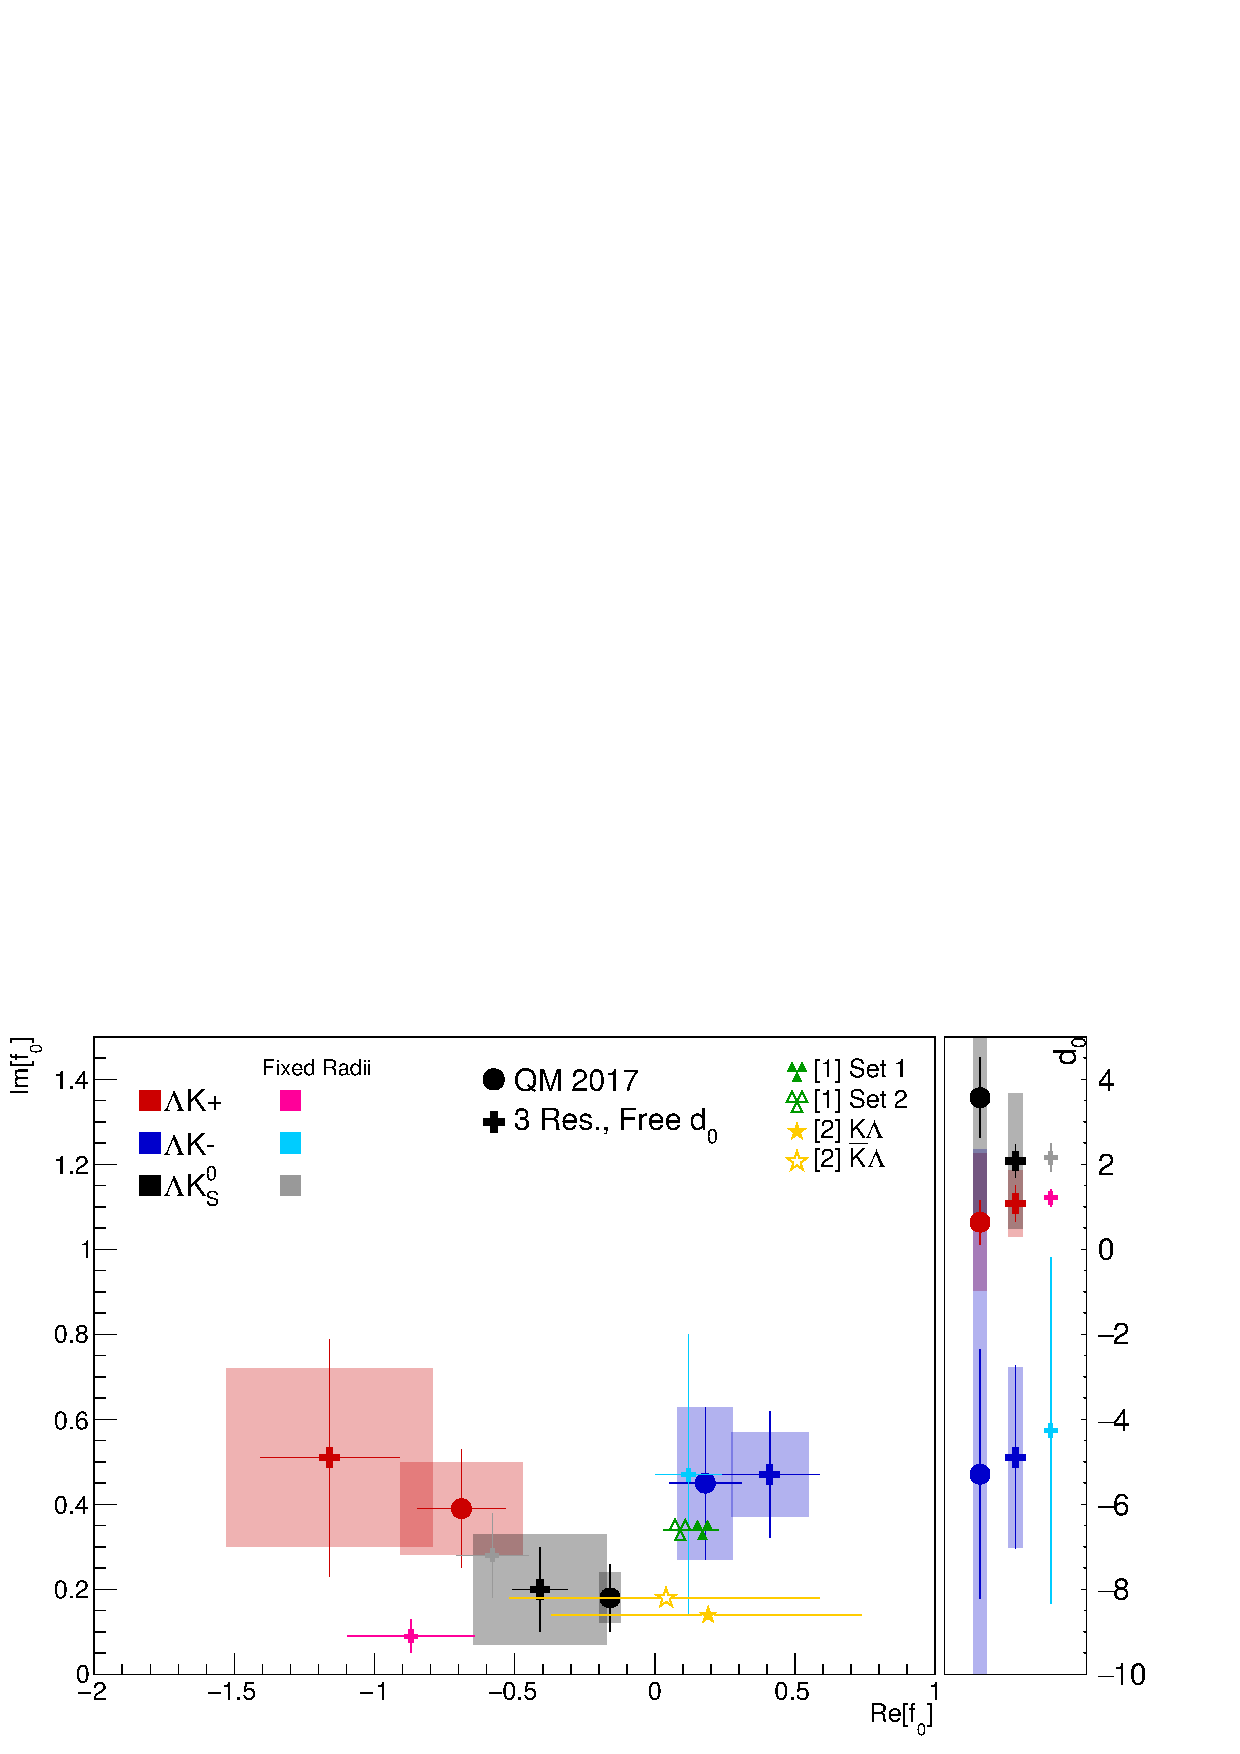
\includegraphics[width=0.49\linewidth]{/home/jesse/Analysis/FemtoAnalysis/LamKPublication/Figures/20171227/PDF/CompareAllReF0vsImF0AcrossAnalyses_3Res_10and3SeparateOnly_FreeD0Only_wFixedRadiiResults_wScattLenPredictions.pdf}}
  %%----start of second subfigure---  
  \subfigure[Extracted $\lambda$ vs Radius results, for the 0-10\% centrality bin, for all of our \LamKchP systems.]{
    \label{fig:LamKFitParams:b}
    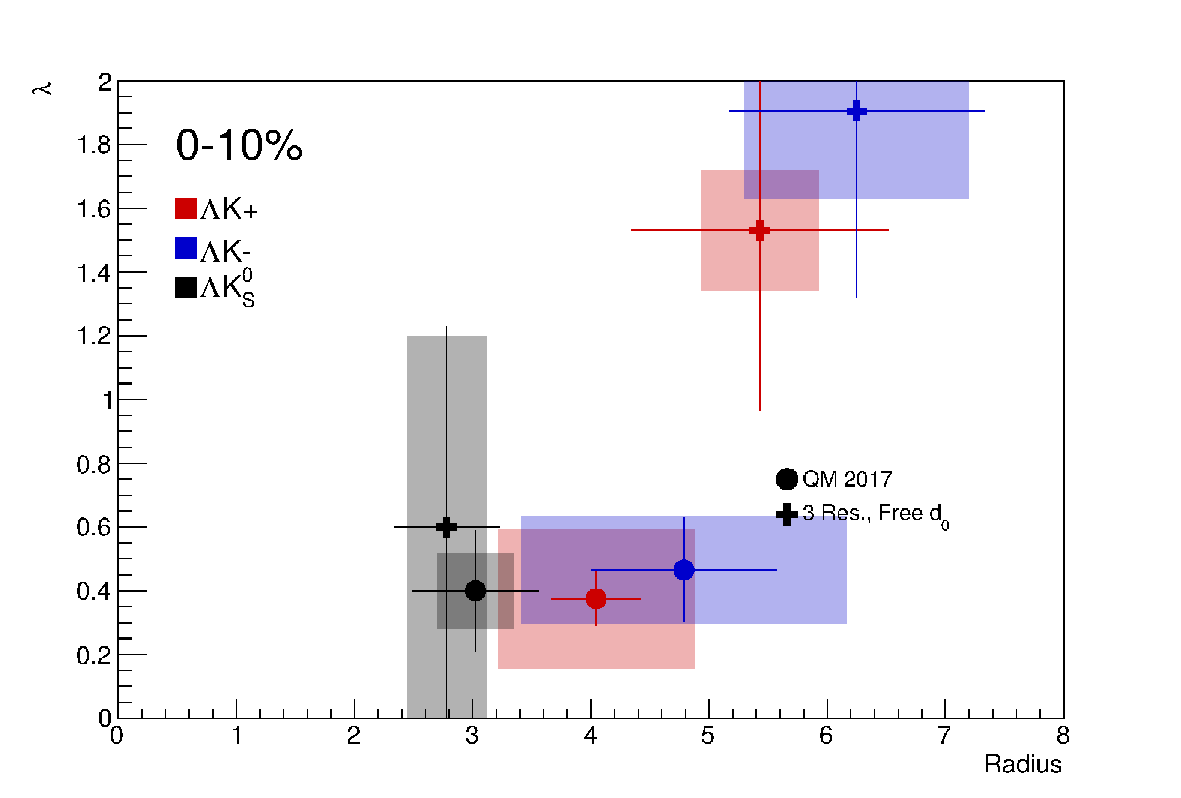
\includegraphics[width=0.49\linewidth]{/home/jesse/Analysis/FemtoAnalysis/LamKPublication/Figures/20171227/PDF/CompareAllRadiusvsLambdaAcrossAnalyses_0010_3Res_10and3SeparateOnly_FreeD0Only.pdf}}
  \\  
  %%----start of third subfigure---  
  \subfigure[Extracted $\lambda$ vs Radius results, for the 10-30\% centrality bin, for all of our \LamKchP systems.]{
    \label{fig:LamKFitParams:c}
    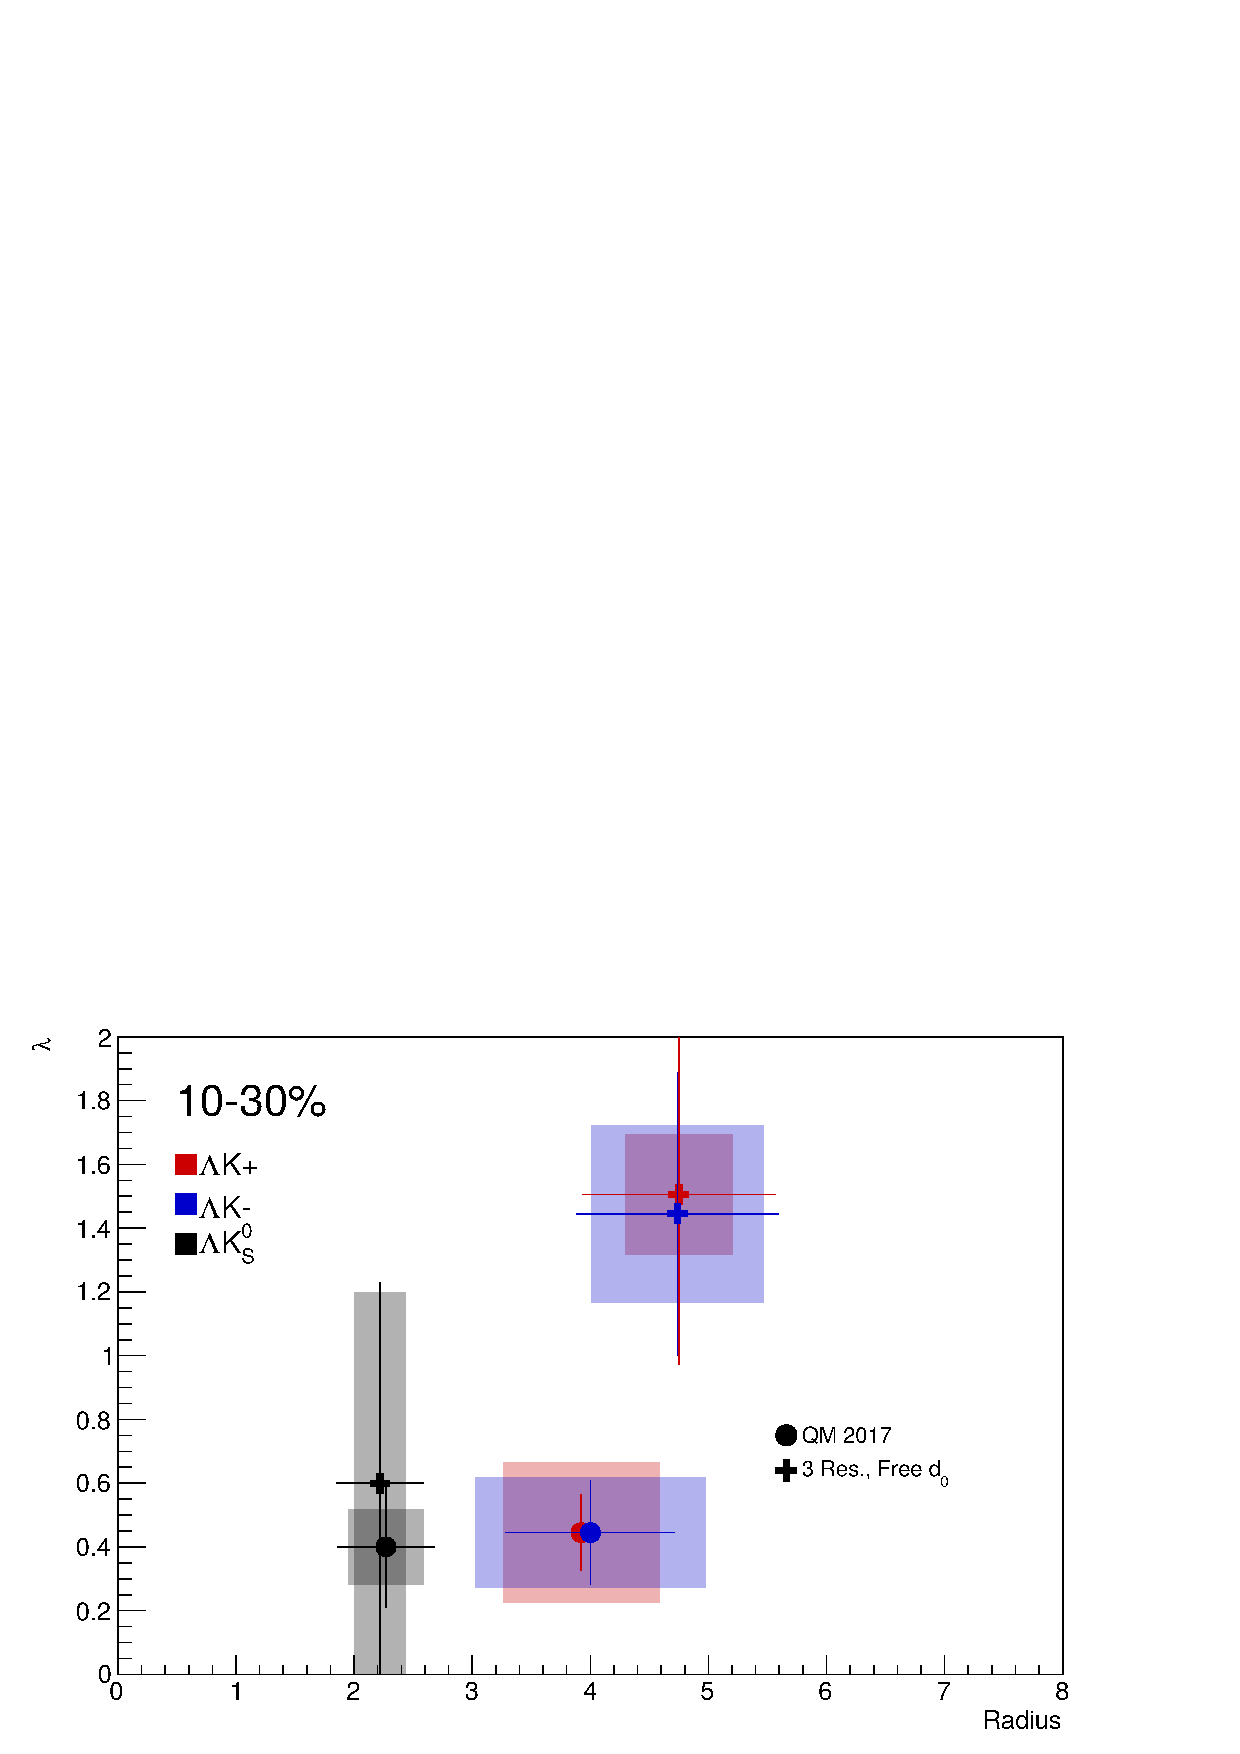
\includegraphics[width=0.49\linewidth]{/home/jesse/Analysis/FemtoAnalysis/LamKPublication/Figures/20171227/PDF/CompareAllRadiusvsLambdaAcrossAnalyses_1030_3Res_10and3SeparateOnly_FreeD0Only.pdf}}    
  %%----start of fourth subfigure---  
  \subfigure[Extracted $\lambda$ vs Radius results, for the 30-50\% centrality bin, for all of our \LamKchP systems.]{
    \label{fig:LamKFitParams:d}
    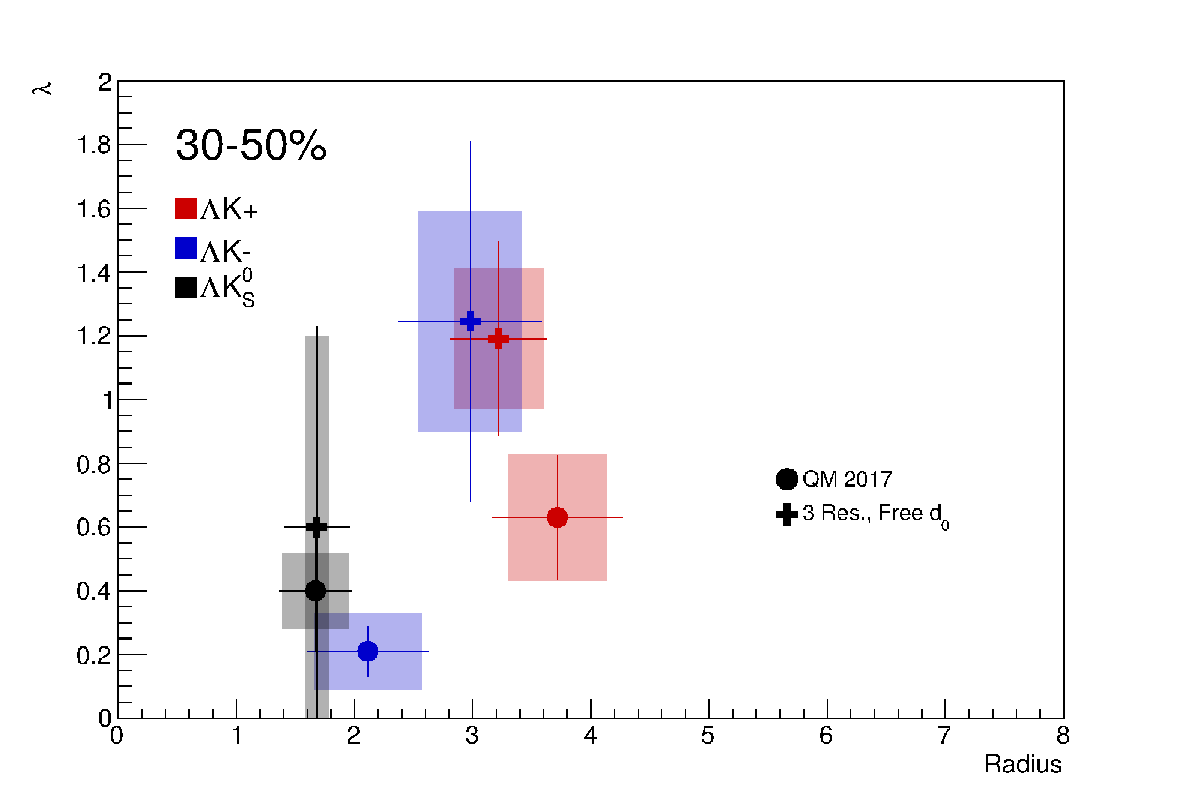
\includegraphics[width=0.49\linewidth]{/home/jesse/Analysis/FemtoAnalysis/LamKPublication/Figures/20171227/PDF/CompareAllRadiusvsLambdaAcrossAnalyses_3050_3Res_10and3SeparateOnly_FreeD0Only.pdf}}    
  %%----overall caption----
  \caption{Extracted fit results for all of our $\Lambda$K systems across all studied centrality bins (0-10\%, 10-30\%, 30-50\%).  The plots show results including no residuals (circles), 10 residual pairs (X), and 3 residual pairs (+).  Note, \LamKchP on the plot is shorthand for \LamKchP and \ALamKchM, and similar for the others.  In Fig. \ref{fig:LamKFitParams:a}, the lighter color markers (pink, sky blue, gray) show the extracted parameters when we fix the radii to roughly align with the $m_{\mathrm{T}}$-scaling plot (Fig. \ref{fig:mTScalingOfRadii_NoRes}).  Additionally, the green \cite{Liu:2006xja} and yellow \cite{Mai:2009ce} points show theoretical predictions made using chiral perturbation theory.}  
  \label{fig:LamKFitParams}
\end{figure}




\begin{figure}[b]
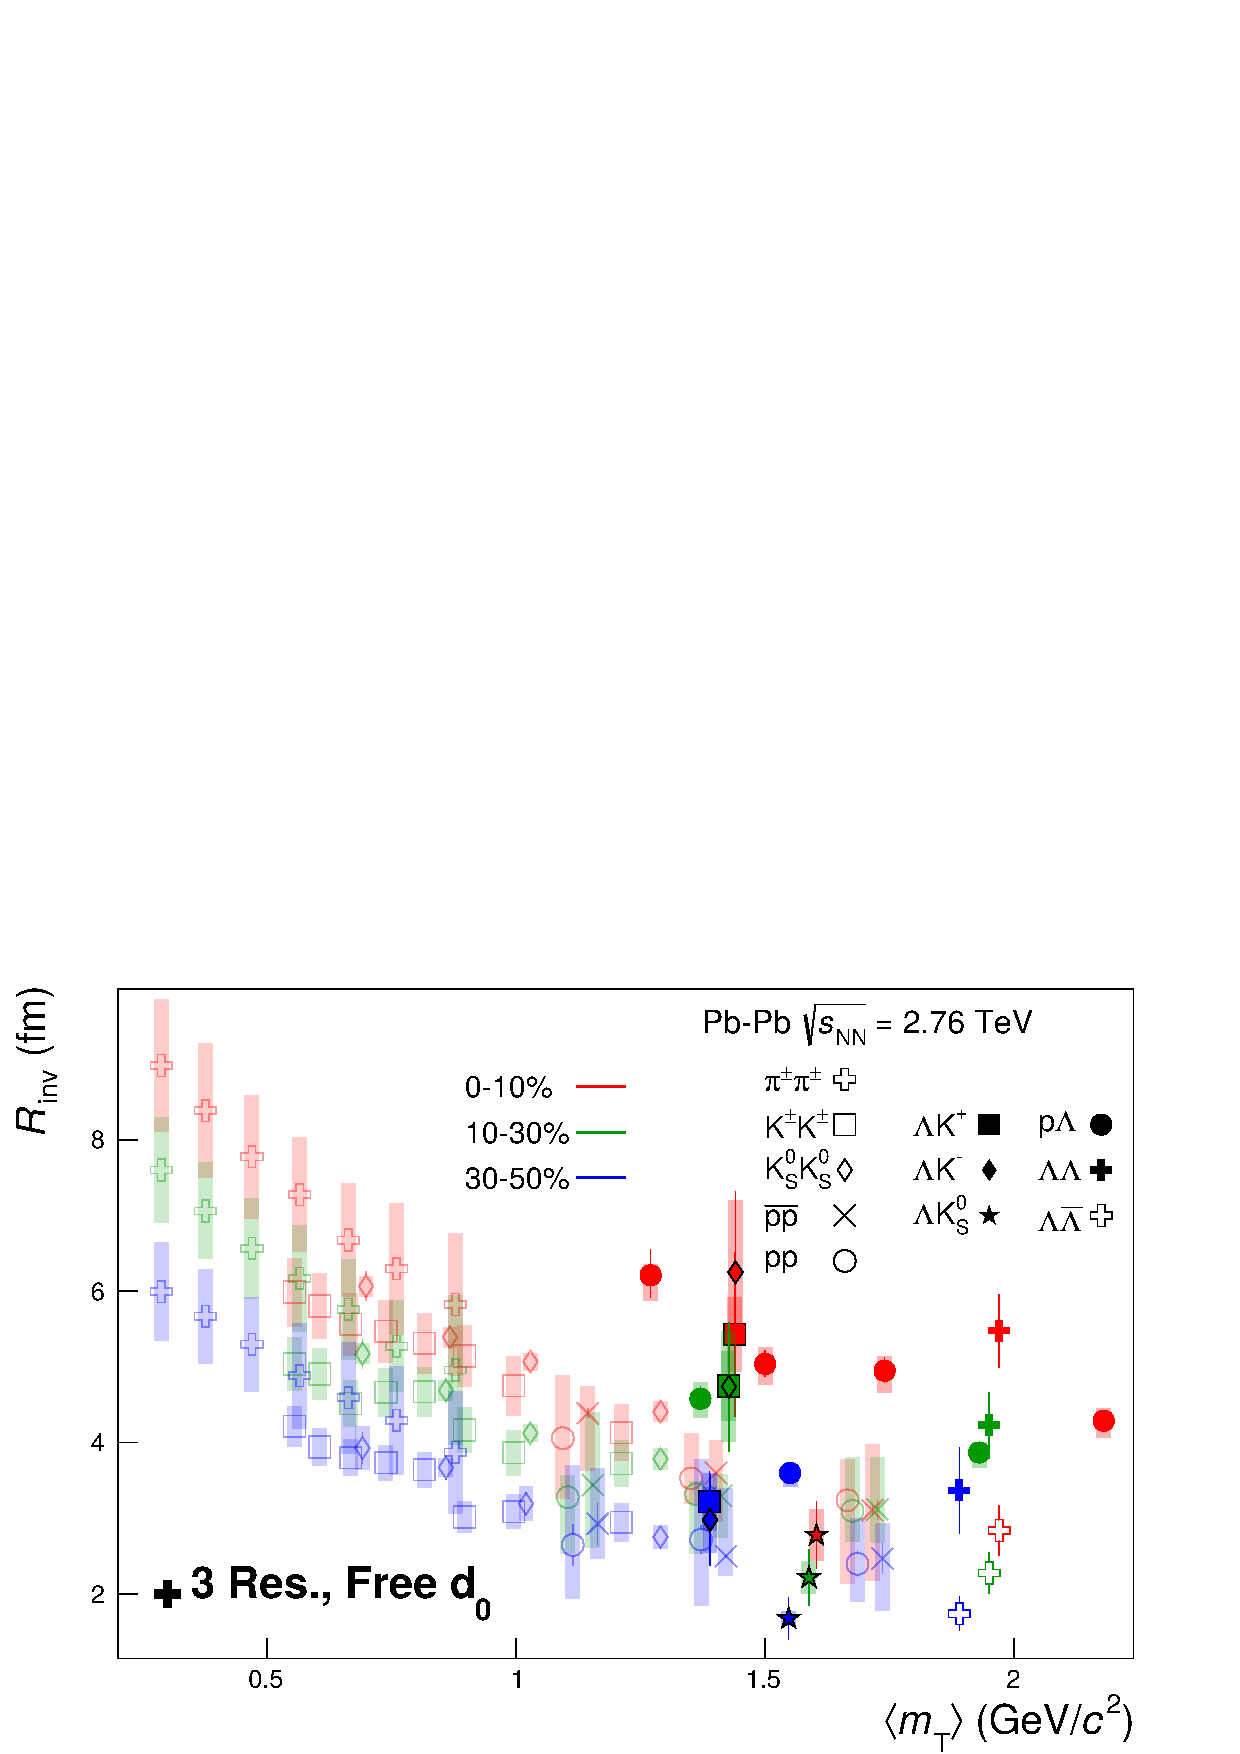
\includegraphics[width=1.0\textwidth]{/home/jesse/Analysis/FemtoAnalysis/LamKPublication/Figures/20171227/PDF/mTscaling_MinvCalc_OutlinedPoints_OthersTransparent_3Res_FreeD0.pdf}% Here is how to import EPS art
\caption{\label{fig:mTScalingOfRadii_NoRes} A figure caption. The figure captions are
automatically numbered.}
\end{figure}



\section{Summary}
\label{sec:Summary}
We did physics, and we found physics.

%%%%% acknowledgements
\newenvironment{acknowledgement}{\relax}{\relax}
\begin{acknowledgement}
\section*{Acknowledgements}
%\input{acknowledgements.tex}    %%%%%%% done by webmaster team
\end{acknowledgement}

%%%%%%%% Bibliography (In case of using bibtex generate the bbl requested by arXiv)
\bibliographystyle{utphys}   % Remember we use title in the biblio
\bibliography{LamK_bibfile}
%\input {bibliography.tex}  

%%%%%%%%% appendix with author list
\newpage
\appendix
%
%\input{}               %%%%%%%%%%% put your appendices here
%


\pagestyle{empty}
\begin{landscape}

\section{$\lambda$ Parameters}
\label{App:LamParams}

\begin{table}[htbp]
 \centering
 \renewcommand{\arraystretch}{1.2}
 \resizebox{\paperwidth}{!}{
 \begin{tabular}{|c|cV{5.0}c|cV{5.0}c|cV{5.0}c|cV{5.0}c|cV{5.0}c|c|}
  \multicolumn{2}{c}{\LamKchP residuals} & \multicolumn{2}{c}{\ALamKchM residuals} & \multicolumn{2}{c}{\LamKchM residuals} & \multicolumn{2}{c}{\ALamKchP residuals} & \multicolumn{2}{c}{\LamKs residuals} & \multicolumn{2}{c}{\ALamKs residuals} \\
  \hline
  \textbf{Pair System} & \textbf{$\lambda$ value} & \textbf{Pair System} & \textbf{$\lambda$ value} & \textbf{Pair System} & \textbf{$\lambda$ value} & \textbf{Pair System} & \textbf{$\lambda$ value} & \textbf{Pair System} & \textbf{$\lambda$ value} & \textbf{Pair System} & \textbf{$\lambda$ value} \\
  \hlineB{3.0}
  \multicolumn{12}{|c|}{3 Residuals} \\
  \hlineB{3.0}
  $\Lambda$K$^{+}$ & 0.154 & $\bar{\Lambda}$K$^{-}$ & 0.158 & $\Lambda$K$^{-}$ & 0.154 & $\bar{\Lambda}$K$^{+}$ & 0.158 & $\Lambda$K$^{0}_{\mathrm{S}}$ & 0.165 & $\bar{\Lambda}$K$^{0}_{\mathrm{S}}$ & 0.169 \\
  $\Sigma^{0}$K$^{+}$ & 0.099 & $\bar{\Sigma}^{0}$K$^{-}$ & 0.102 & $\Sigma^{0}$K$^{-}$ & 0.099 & $\bar{\Sigma}^{0}$K$^{+}$ & 0.103 & $\Sigma^{0}$K$^{0}_{\mathrm{S}}$ & 0.107 & $\bar{\Sigma}^{0}$K$^{0}_{\mathrm{S}}$ & 0.111 \\
  $\Xi^{0}$K$^{+}$ & 0.072 & $\bar{\Xi}^{0}$K$^{-}$ & 0.067 & $\Xi^{0}$K$^{-}$ & 0.071 & $\bar{\Xi}^{0}$K$^{+}$ & 0.068 & $\Xi^{0}$K$^{0}_{\mathrm{S}}$ & 0.077 & $\bar{\Xi}^{0}$K$^{0}_{\mathrm{S}}$ & 0.073 \\
  $\Xi^{-}$K$^{+}$ & 0.069 & $\bar{\Xi}^{+}$K$^{-}$ & 0.065 & $\Xi^{-}$K$^{-}$ & 0.068 & $\bar{\Xi}^{+}$K$^{+}$ & 0.066 & $\Xi^{-}$K$^{0}_{\mathrm{S}}$ & 0.075 & $\bar{\Xi}^{+}$K$^{0}_{\mathrm{S}}$ & 0.071 \\
  Other & 0.558 & Other & 0.560 & Other & 0.561 & Other & 0.557 & Other & 0.528 & Other & 0.528 \\
  Fakes & 0.048 & Fakes & 0.048 & Fakes & 0.048 & Fakes & 0.048 & Fakes & 0.048 & Fakes & 0.048 \\
  \hlineB{3.0}  
  \multicolumn{12}{|c|}{10 Residuals} \\
  \hlineB{3.0}
  $\Lambda$K$^{+}$ & 0.154 & $\bar{\Lambda}$K$^{-}$ & 0.158 & $\Lambda$K$^{-}$ & 0.154 & $\bar{\Lambda}$K$^{+}$ & 0.158 & $\Lambda$K$^{0}_{\mathrm{S}}$ & 0.165 & $\bar{\Lambda}$K$^{0}_{\mathrm{S}}$ & 0.169 \\
  $\Sigma^{0}$K$^{+}$ & 0.099 & $\bar{\Sigma}^{0}$K$^{-}$ & 0.102 & $\Sigma^{0}$K$^{-}$ & 0.099 & $\bar{\Sigma}^{0}$K$^{+}$ & 0.103 & $\Sigma^{0}$K$^{0}_{\mathrm{S}}$ & 0.107 & $\bar{\Sigma}^{0}$K$^{0}_{\mathrm{S}}$ & 0.111 \\
  $\Xi^{0}$K$^{+}$ & 0.072 & $\bar{\Xi}^{0}$K$^{-}$ & 0.067 & $\Xi^{0}$K$^{-}$ & 0.071 & $\bar{\Xi}^{0}$K$^{+}$ & 0.068 & $\Xi^{0}$K$^{0}_{\mathrm{S}}$ & 0.077 & $\bar{\Xi}^{0}$K$^{0}_{\mathrm{S}}$ & 0.073 \\
  $\Xi^{-}$K$^{+}$ & 0.069 & $\bar{\Xi}^{+}$K$^{-}$ & 0.065 & $\Xi^{-}$K$^{-}$ & 0.068 & $\bar{\Xi}^{+}$K$^{+}$ & 0.066 & $\Xi^{-}$K$^{0}_{\mathrm{S}}$ & 0.075 & $\bar{\Xi}^{+}$K$^{0}_{\mathrm{S}}$ & 0.071 \\
  $\Sigma^{*+}$K$^{+}$ & 0.046 & $\bar{\Sigma}^{*-}$K$^{-}$ & 0.046 & $\Sigma^{*+}$K$^{-}$ & 0.046 & $\bar{\Sigma}^{*-}$K$^{+}$ & 0.046 & $\Sigma^{*+}$K$^{0}_{\mathrm{S}}$ & 0.050 & $\bar{\Sigma}^{*-}$K$^{0}_{\mathrm{S}}$ & 0.050 \\
  $\Sigma^{*-}$K$^{+}$ & 0.042 & $\bar{\Sigma}^{*+}$K$^{-}$ & 0.045 & $\Sigma^{*-}$K$^{-}$ & 0.041 & $\bar{\Sigma}^{*+}$K$^{+}$ & 0.045 & $\Sigma^{*-}$K$^{0}_{\mathrm{S}}$ & 0.045 & $\bar{\Sigma}^{*+}$K$^{0}_{\mathrm{S}}$ & 0.049 \\
  $\Sigma^{*0}$K$^{+}$ & 0.042 & $\bar{\Sigma}^{*0}$K$^{-}$ & 0.040 & $\Sigma^{*0}$K$^{-}$ & 0.041 & $\bar{\Sigma}^{*0}$K$^{+}$ & 0.041 & $\Sigma^{*0}$K$^{0}_{\mathrm{S}}$ & 0.045 & $\bar{\Sigma}^{*0}$K$^{0}_{\mathrm{S}}$ & 0.044 \\
  $\Lambda$K$^{*0}$ & 0.039 & $\bar{\Lambda}\bar{\mathrm{K}}^{*0}$ & 0.041 & $\Lambda\bar{\mathrm{K}}^{*0}$ & 0.039 & $\bar{\Lambda}$K$^{*0}$ & 0.041 & $\Lambda$K$^{*0}$ & 0.019 & $\bar{\Lambda}$K$^{*0}$ & 0.020 \\
  $\Sigma^{0}$K$^{*0}$ & 0.035 & $\bar{\Sigma}^{0}\bar{\mathrm{K}}^{*0}$ & 0.036 & $\Sigma^{0}\bar{\mathrm{K}}^{*0}$ & 0.035 & $\bar{\Sigma}^{0}$K$^{*0}$ & 0.036 & $\Sigma^{0}$K$^{*0}$ & 0.017 & $\bar{\Sigma}^{0}$K$^{*0}$ & 0.017 \\
  $\Xi^{0}$K$^{*0}$ & 0.025 & $\bar{\Xi}^{0}\bar{\mathrm{K}}^{*0}$ & 0.024 & $\Xi^{0}\bar{\mathrm{K}}^{*0}$ & 0.025 & $\bar{\Xi}^{0}$K$^{*0}$ & 0.024 & $\Xi^{0}$K$^{*0}$ & 0.012 & $\bar{\Xi}^{0}$K$^{*0}$ & 0.011 \\
  $\Xi^{-}$K$^{*0}$ & 0.024 & $\bar{\Xi}^{+}\bar{\mathrm{K}}^{*0}$ & 0.023 & $\Xi^{-}\bar{\mathrm{K}}^{*0}$ & 0.024 & $\bar{\Xi}^{+}$K$^{*0}$ & 0.023 & $\Xi^{-}$K$^{*0}$ & 0.012 & $\bar{\Xi}^{+}$K$^{*0}$ & 0.011 \\
  Other & 0.305 & Other & 0.305 & Other & 0.308 & Other & 0.301 & Other & 0.329 & Other & 0.326 \\
  Fakes & 0.048 & Fakes & 0.048 & Fakes & 0.048 & Fakes & 0.048 & Fakes & 0.048 & Fakes & 0.048 \\
  \hlineB{3.0}
 \end{tabular}}
 \caption{$\lambda$ values for the individual components of the \LamK correlation functions for the case of 3 and 10 residual contributions.}
 \label{tab:LambdaValues_All}
\end{table}

\end{landscape}
\pagestyle{plain}





\section{The ALICE Collaboration}
\label{app:collab}
%\input{authorlist-preprint.tex}  %%%%%%% done by webmaster team
\end{document}
